\documentclass[a4paper, 12pt]{article}

% \usepackage[utf8]{inputenc}
% \usepackage{tgtermes}
% \usepackage{fouriernc}
\usepackage[T1]{fontenc}
\usepackage[margin=3cm]{geometry}
\usepackage{babel}

\usepackage{biblatex}
\addbibresource{refs.bib}

\usepackage{amssymb}
\usepackage{amsmath}

\usepackage{ebproof}

\usepackage{enumerate}
\usepackage{verbatim}

\usepackage{xcolor}

\usepackage{listings}
\lstset{mathescape=true,
 xleftmargin=.25in}
\usepackage{quiver}

\usepackage[skip=10pt]{parskip}

\newcommand{\N}{\mathbb{N}}
\newcommand{\Z}{\mathbb{Z}}
\newcommand{\Q}{\mathbb{Q}}
\newcommand{\R}{\mathbb{R}}
\newcommand{\C}{\mathbb{C}}
\newcommand{\B}{\mathbb{B}}
\newcommand{\dif}{\mathrm{d}}
\newcommand{\Prop}{\mathit{Prop}}
\newcommand{\type}{\textsc{ Type}}
\newcommand{\Type}{\mathit{Type}}
\newcommand{\Sort}{\mathit{Sort\;}}
\renewcommand{\Prop}{\mathit{Prop}}
\DeclareMathOperator{\Arg}{Arg}
\DeclareMathOperator{\IN}{IN}
\DeclareMathOperator{\LT}{LT}
\newcommand{\la}[1]{\lambda{#1}.\,}


% Kan Danny godt lide
\usepackage[autostyle]{csquotes}
\usepackage{kpfonts}
% \usepackage{inconsolata}
\linespread{1.06}

\usepackage{minted}
\usemintedstyle{tango}
\setminted{fontsize=\footnotesize}
\setminted{breaklines}
\newcommand{\lean}[1]{\mintinline{lean}{#1}}

\usepackage{fontspec}
\setmonofont{JuliaMono}
\setmainfont{Linux Libertine O}
% \setmathfont[Digits, Latin]{Linux Biolinum O}

\usepackage{xcolor}
\usepackage{hyperref}
\hypersetup{%
	pdftitle=Mathematical project in Lean,
	pdfauthor={Andreas Bøgh Poulsen},
	colorlinks,
	linkcolor={red!50!black},
	citecolor={red!50!black},
	urlcolor={red!50!black},
	bookmarksnumbered=true
}

\usepackage[ntheorem]{mdframed}
\usepackage[amsmath,thmmarks,hyperref]{ntheorem}
\usepackage[capitalize]{cleveref}

% Frame for theorems
\definecolor{shadecolor}{gray}{0.93}
\definecolor{rulecolor}{gray}{0.4}
\mdfdefinestyle{thmframed}{%
	%usetwoside=false, % For use with memoir twoside
	skipabove=0.5em plus 0.4em minus 0.2em,
	skipbelow=0.5em plus 0.4em minus 0.2em,
	leftmargin=-7pt, rightmargin=-7pt, innerleftmargin=6pt,
	innerrightmargin=6pt, innertopmargin=6pt, innerbottommargin=3pt,
	% linewidth=1pt, linecolor=rulecolor, backgroundcolor=shadecolor,
  linewidth=1.5pt, linecolor=rulecolor, topline=false, bottomline=false, rightline=false, %leftmargin=1em,
	splittopskip=1.2em minus 0.2em,
	splitbottomskip=0.5em plus 0.2em minus 0.1em,
}
\mdfdefinestyle{thmempty}{
  usetwoside=false, % For use with memoir twoside
	skipabove=0.5em plus 0.4em minus 0.2em,
	skipbelow=0.5em plus 0.4em minus 0.2em,
	leftmargin=-7pt, rightmargin=-7pt, innerleftmargin=6pt,
	innerrightmargin=6pt, innertopmargin=6pt, innerbottommargin=3pt,
	% linewidth=1pt, linecolor=rulecolor, backgroundcolor=shadecolor,
  linewidth=1.5pt, linecolor=rulecolor, topline=false, bottomline=false, rightline=false,
	splittopskip=1.2em minus 0.2em,
	splitbottomskip=0.5em plus 0.2em minus 0.1em,
}

% New theorem style with a dot
\makeatletter
\newtheoremstyle{changedot}%
  {\item[\hskip\labelsep \theorem@headerfont ##2~~$\cdot$~~##1\theorem@separator]}%
  {\item[\hskip\labelsep \theorem@headerfont ##2~~$\cdot$~~##1\ (##3)\theorem@separator]}

\newtheoremstyle{changedotbreak}%
  {\item\hbox to \textwidth{\theorem@headerfont ##2~~$\cdot$~~##1\theorem@separator\hfill}}%
  {\item\hbox to \textwidth{\theorem@headerfont ##2~~$\cdot$~~##1\
      (##3)\theorem@separator\hfill}}
\makeatother

\theoremstyle{changedot}
\theoremseparator{.}
% \newmdtheoremenv[style=thmframed]{theorem}{Theorem}[section]
% \newmdtheoremenv[style=thmframed]{proposition}[theorem]{Proposition}
% \newmdtheoremenv[style=thmframed]{lemma}[theorem]{Lemma}
% \newmdtheoremenv[style=thmframed]{corollary}[theorem]{Corollary}
\newmdtheoremenv[style=thmempty]{theorem}{Theorem}[section]
\newmdtheoremenv[style=thmempty]{proposition}[theorem]{Proposition}
\newmdtheoremenv[style=thmempty]{lemma}[theorem]{Lemma}
\newmdtheoremenv[style=thmempty]{corollary}[theorem]{Corollary}

\theorembodyfont{\normalfont}
%\theoremsymbol{\ensuremath{\triangle}}
\newmdtheoremenv[style=thmframed]{definition}[theorem]{Definition}

\theoremstyle{changedotbreak}
\newmdtheoremenv[style=thmframed]{definitionbreak}[theorem]{Definition}

\theoremstyle{nonumberplain}
\theoremheaderfont{\normalfont\itshape}
\theorembodyfont{\normalfont}
\theoremsymbol{\ensuremath{\square}}
\newtheorem{proof}{Proof}

\Crefname{theorem}{Theorem}{Theorems}
\Crefname{proposition}{Proposition}{Propositions}
\Crefname{lemma}{Lemma}{Lemmata}
\Crefname{corollary}{Corollary}{Corollaries}
\Crefname{definition}{Definition}{Definitions}

\crefformat{equation}{(#2#1#3)}

% / Kan Danny godt lide

% \usepackage[eng,exjobb]{KTHEEtitlepage}

\title{Mathematical project in \textsf{L$\exists \forall\N$}\\{\large \textsc{An innocent mathematicians guide to lean}}}
\author{Andreas Bøgh Poulsen, studienummer: 201805425}

\newcommand*{\titleGM}{%\begingroup % Create the command for including the title page in the document
%\hbox{ % Horizontal box
\hspace*{0.2\textwidth} % Whitespace to the left of the title page
\rule{1pt}{\textheight} % Vertical line
\hspace*{0.05\textwidth} % Whitespace between the vertical line and title page text
\parbox[b]{0.75\textwidth}{ % Paragraph box which restricts text to less than the width of the page
{\noindent\Huge\bfseries  Mathematical project in \textsf{L$\exists \forall\N$}\\{\large \textsc{An innocent mathematicians guide to lean}}\\}\\[2\baselineskip] % Title
{\large \textit{Andreas Bøgh Poulsen \hfill 201805425 }}\\%[1\baselineskip]
% {\large  } \\[4\baselineskip] % Tagline or further description
{\large } % Author name
\parbox[b][0pt]{0.5\textwidth}{
  \hspace{2cm}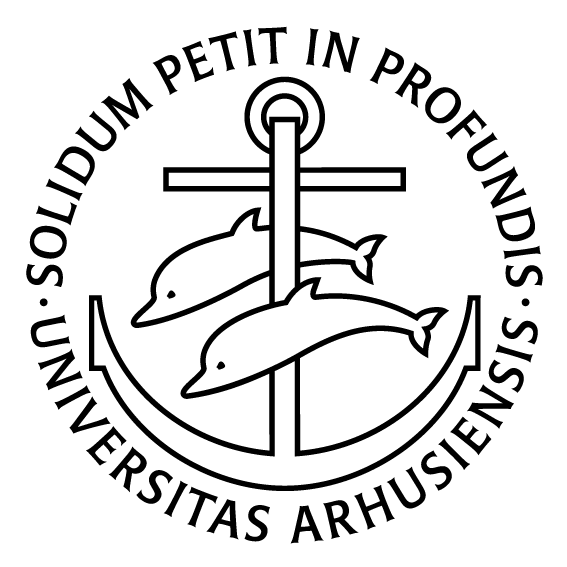
\includegraphics[width=0.5\textwidth]{ausegl_sort.png}
  \vspace{-10cm}
}

% \begin{centering}
  % 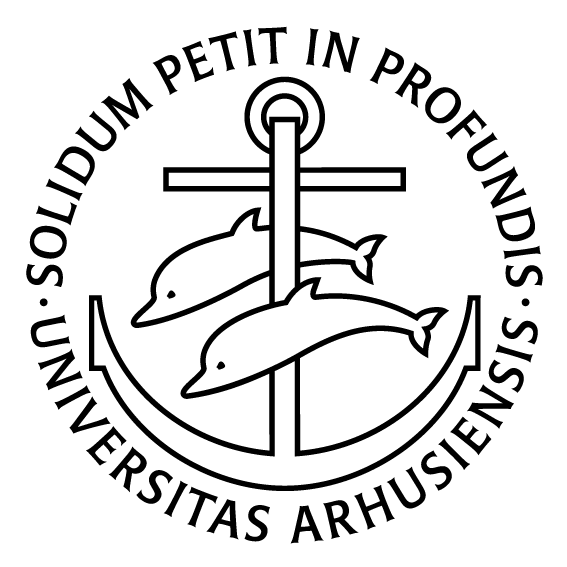
\includegraphics[width=0.5\textwidth]{ausegl_sort.png}
% \end{centering}
\vspace{0.5\textheight} % Whitespace between the title block and the publisher
\vfill
{\noindent Supervisor: Niels Lauritzen \hspace{2.5cm} 
\includegraphics{AU_logo.png}  }\\[\baselineskip] % Publisher and logo
}%}
% \endgroup
}

\begin{document}
% \maketitle
\titleGM
% \vfill
% Vejleder: Niels Lauritzen
% \strut\hfill
% 
\includegraphics[right]{AU_logo.png}
\newpage
\tableofcontents

\newpage

\section*{Introduction}
The following is a project, in which I try to learn how to do formalized mathematics, using Lean as my proof checker. This document is a report on my learnings and is intended as a resource for other mathematicians, who may wish to learn about Lean.

The first section covers a variant of the type theory used in Lean. In it, I build a mathematical foundation, on which to base your understanding of Lean. The second section introduces Lean as a tool to assist the tedious work of doing formalized mathematics. Here, I also showcase some of the ``engineering'' aspects of Lean, which are needed to scale a formalism to the state of modern mathematics. In particular, I highlight the use of type classes, which will be needed in section 3. The third section is dedicated to walking through a worked example, which is the development of Gröbner bases for polynomial rings over fields. This is to show the work required to bring a modern algebraic theory into Lean. It will also serve as a reference example for others, who wish to formalize non-trivial mathematics in Lean.

\section{Martin-Löf dependent type theory}\label{sec:tt}
Dependent type theory is a logical theory, comparable to first-order logic. Similarly to how we usually think we do mathematics in first-order logic with ZFC set theory on top, we can translate our mathematical theories into other logical theories. In this section, I'll explain how dependent type theory works as a formal system. The development will largely follow the exposition of \cite{rijke2022introduction}.

We'll build a dependent type theory, which is similar to the one used by Lean. The goal is not to match the calculus of inductive constructions (which is used in Lean), but rather to develop a theory together, to see how and why the choices Lean has made, make sense. If you're only interested in learning Lean, feel free to skip this section.

\subsection{Intuition and how to read the notation}
The following development may seem very notation-heavy and needlessly abstract, so here's a little primer: Suppose I have three functions (or morphisms)
\begin{align*}
  f &: A \to B \\
  g &: A \to C \\
  h &: B \to C
\end{align*}

The the composition $h \circ f : A \to C$ make sense, but the composition $h \circ g$ doesn't. Keeping track of domains and codomains in this small example is not a problem, but when more functions get involved, it can become unwieldy. This is where a type-checking compiler, as found in programming languages like Java and Haskell, can help.

Similarly, if we have three propositions
\begin{align*}
  p_{1} &= P \implies Q \\
  p_{2} &= P \implies R \\
  p_{3} &= Q \implies R
\end{align*}

have can deduce $P \implies R$ from $p_{1}$ and $p_{3}$, but we cannot deduce that from $p_{1}$ and $p_{2}$. This is similar to the situation above. In fact, we translate our propositions directly into functions and get a compiler to check it for us.

Now, most propositions are not fixed statements, they are parameterized by variables, for example $p_{4} = x \le 0$. Since the truth of this proposition is dependent on the element $x$, we can't translate it into any fixed type. So we extend the type theory of our programming language, so that types can depend on variables, then build a type-checker for this type theory, and then we get a checker for our propositions.

\subsubsection{Deduction rules}

The rules for our language are given by deduction rules. There are two types of deduction rules: typing rules and evaluation rules. The typing rules are only needed by the type checker. They are statements of the form \textit{``if $f : A \to B$ and $g : B \to C$ are functions with given domains and codomains, then $g \circ f : A \to C$ is a function with the given domain and codomain.''} Strictly speaking, this is all we need to formulate mathematics, as we only need the type checker. However, it will turn out to be useful to have an actual programming language. This means we need to define what $g \circ f$ does. This is given by an evaluation rule: \textit{``if $a \in A$ is an element and $f : A \to B$ and $g : B \to C$ are functions with given domains and codomains, then $(g \circ f)(a) = g(f(a))$.''} This tells us how to evaluate the terms we build. In the text below, rules that end in $A \type$ or $a : A$ are typing rules, and rules like $f(x) \doteq y$ are evaluation rules.

\subsection{Inference rules}
An inference rule is on the form

\begin{prooftree}
  \hypo{\Gamma \vdash P}
  \hypo{\Gamma \vdash Q}
  \infer2[$\land$-intro]{\Gamma \vdash P \land Q}
\end{prooftree}

which is read as follows: if we, in a context $\Gamma$, can prove $P$ and in the same context can prove $Q$, then we can prove $P \land Q$ in the context $\Gamma$.

The defining feature of {\emph type} theory is, that every element has a type. Thus the above is meaningless, as $P$ and $Q$ have no type. Compare this to ZFC, where everything is either a proposition from first-order logic, or a set. This leads to weird statements like $0 \in 1$, which is well-posed since everything is a set but does not carry meaning in our ``usual'' way of doing mathematics. Type theory asks that every element has a type. This is particularly helpful when doing computerized proofs, as it helps the proof-checker catch weird statements like $0 \in 1$. Since $1$ has the type of a natural number and not the type of a set, Lean can give an error, instead of silently trying to prove what may well have been a typo.

In type theory, the above rewrite rule would look like this:

\begin{prooftree}
  % \hypo{\Gamma \vdash \mathit{Prop} \type}
  \hypo{\Gamma \vdash P : \mathit{Prop}}
  \hypo{\Gamma \vdash Q : \mathit{Prop}}
  \infer2[$\land$-intro]{\Gamma \vdash P \land Q : \Prop}
\end{prooftree}

Everything is read the same, except $P : \Prop$ is read ``$P$ has type $\Prop$''. $\Prop$ is the type of propositions. I will not spend too much time going through every single inference rule. I will, however, introduce the defining features of dependent type theory: dependent types, and show how they are used.

\begin{definition}
  Type theory has four different \textit{judgments}.
  \begin{enumerate}
    \item $\Gamma \vdash A \type$ says $A$ is a well-formed type in context $\Gamma$.
    \item $\Gamma \vdash A \doteq B \type$ says $A$ and $B$ are judgementally equal types in context $\Gamma$.
    \item $\Gamma \vdash a : A$ says $a$ is an element of type $A$ in context $\Gamma$.
    \item $\Gamma,\, a:A,\, b:A \vdash a \doteq b : A$ says $a$ and $b$ both have type $A$ and are judgementally equal.
  \end{enumerate}
\end{definition}

As we would expect, there are axioms making judgemental equality an equivalence relation:

\begin{align*}
  &\begin{prooftree}
    \hypo{\Gamma \vdash a : A}
    \infer1{\Gamma \vdash a \doteq a : A}
  \end{prooftree}
  &
  \begin{prooftree}
    \hypo{\Gamma \vdash a \doteq b : A}
    \infer1{\Gamma \vdash b \doteq a : A}
  \end{prooftree}
  &
  &\begin{prooftree}
    \hypo{\Gamma \vdash a \doteq b : A}
    \hypo{\Gamma \vdash b \doteq c : A}
    \infer2{\Gamma \vdash a \doteq c : A}
  \end{prooftree}
\end{align*}

and similarly for types. There is also a rule stating that you can substitute judgementally equal elements anywhere.

Judgemental equality is actually a very strong equality, and many objects we usually consider equal, cannot be proven judgementally equal. Later we'll introduce a weaker equality, that captures better our usual understanding of equality. Stay tuned, the formulation may surprise you.

We need to introduce dependent types as well as functions, before we can get going.

\begin{definition}
  A \textit{dependent type} is a type of the form $\Gamma, x : A \vdash B(x) \type$ with a rule letting us assume elements of that type:

  \begin{center}
    \begin{prooftree}
      \hypo{\Gamma, x : A \vdash B(x) \type}
      \infer1{\Gamma, x : A, b : B(x) \vdash b : B(x)}
    \end{prooftree}
  \end{center}

  When $B(x)$ is independent of $x$ we simply write $B$. In that case:
  \begin{center}
    \begin{prooftree}
      \hypo{\Gamma \vdash B \type}
      \infer1{\Gamma, b : B \vdash b : B}
    \end{prooftree}
  \end{center}

  Every element has a unique type, up to judgemental equality.

  A \textit{section} of a dependent type $B(x)$ is an element $\Gamma, x : A \vdash b : B(x)$.
\end{definition}

Note that for different $x : A$ in the context, $B(x)$ may be different type. Using dependent types we can introduce functions:

\begin{definition}
  A \textit{function type} is the type of sections of a dependent type $B(x)$, given by the following introduction rules:

  \begin{align*}
    &\begin{prooftree}
      \hypo{\Gamma, x : A \vdash B(x) \type}
      \infer1{\Gamma \vdash \Pi_{x:A} B(x) \type}
    \end{prooftree}
      &
    &\begin{prooftree}
      \hypo{\Gamma, x : A \vdash b(x) : B(x)}
      \infer1{\Gamma \vdash \la x b(x) : \Pi_{x:A} B(x)}
    \end{prooftree}
  \end{align*}

  and has the following evaluation rules:

  \begin{align*}
    &\begin{prooftree}
      \hypo{\Gamma \vdash f : \Pi_{x:A} B(x)}
      \infer1{\Gamma, x : A \vdash f(x) : B(x)}
    \end{prooftree}
    &
    &\begin{prooftree}
      \hypo{\Gamma, x : A \vdash b(x) : B(x)}
      \infer1{\Gamma, x : A \vdash (\la y b(y))(x) \doteq b(x) : B(x)}
    \end{prooftree}
  \end{align*}

\end{definition}

\textit{Remark.} Not all types are dependent. If $B(x)$ is independent of $x$ we will just write functions as $A \to B$. This arrow binds stronger that $\Pi$, so that $\Pi_{a:A}\, B \to C$ is read as $\Pi_{a:A}\, (A \to B)$.

\subsection{Logic in type theory}
We now have the building blocks to start formulating usual logic in dependent type theory. The basic idea is to interpret types as propositions. A proof of a proposition corresponds to an element of a type. Thus a false proposition is a type without any elements, and a true proposition is a type with at least one element. We can introduce canonical false and true propositions:

\begin{definition}
  The types of false and true.

  The empty type (false) is given by
\begin{align*}
  \begin{prooftree}
    \infer0{\vdash \emptyset \type}
  \end{prooftree} & &
  \begin{prooftree}
    \infer0{\vdash ind_{\emptyset} : \Pi_{x:\emptyset} P(x)}
  \end{prooftree}
\end{align*}

and the unit type (true) is given by
\begin{align*}
  \begin{prooftree}
    \infer0{\vdash \mathbf{1} \type}
  \end{prooftree} & &
                    \begin{prooftree}
                      \infer0{\vdash \bullet : \mathbf 1}
                      \end{prooftree}& &
                      \begin{prooftree}
                        \infer0{\vdash ind_{\mathbf 1} : P(\bullet) \to \Pi_{x : \mathbf 1}\, P(x)}
                      \end{prooftree}
  \end{align*}

\end{definition}
\textit{Remark.} The functions $ind_{\emptyset}$ and $ind_{\mathbf 1}$ are called induction functions or induction rules. They govern the behaviour of these and all our future types.

So $\emptyset$ is a false proposition, and $\mathbf 1$ is a true proposition, with the proof $\bullet : \mathbf 1$. What would other logical operators look like in this interpretation? Implication simply becomes a function. $f : A \to B$ says ``f takes an element of $A$ and produces an element of $B$'' or as propositions ``$f$ takes a proof of $A$ and produces a proof of $B$'', which is exactly what an implication does.

In this light, the induction rule of $\emptyset$ states, that given a proof of false, we can prove everything about that element. In particular, $P(x)$ doesn't have to depend on $x$, så given a proof of false, we can prove anything! The induction principle for $\mathbf 1$ is comparatively boring, stating that if something is true about $\bullet$, then it's true about every element of $\mathbf 1$. I other words: if something is true assuming true, and we have a proof of true, that something is true.

We can interpret something being false $\neg A$ as the type $A \to \emptyset$. Then ``$A$ is false'' translates to ``assuming $A$, I can prove false''. We can then prove the statement $(A \implies B) \implies (\neg B \implies \neg A)$. In type theory, this translates to $(A \to B) \to ((B \to \emptyset) \to (A \to \emptyset))$. The construction is as follows:

\begin{theorem}
  $(A \implies B) \implies (\neg B \implies \neg A)$
\end{theorem}
\begin{proof}
  We construct an element of the desired type:
\begin{center}
  \begin{prooftree}
    \hypo{\Gamma \vdash A \type}
    \infer1{\Gamma, a : A \vdash a : A}
    \hypo{\Gamma \vdash A \type}
    \infer1{\Gamma, a : A \vdash a : A}
    \hypo{\Gamma \vdash B \type}
    \infer2{\Gamma \vdash A \to B \type}
    \infer1{\Gamma, h : A \to B \vdash h : A \to B}
    \infer2{\Gamma, a : A, h : A \to B \vdash h(a) : B}
    \hypo{\Gamma \vdash B \type}
    \infer1{\Gamma, b : B \vdash b : B}
    \infer0{\vdash \emptyset \type}
    \infer2{\Gamma \vdash B \to \emptyset \type}
    \infer1{\Gamma, f : B \to \emptyset \vdash f : B \to \emptyset}
    \infer2{\Gamma, a : A, f : B \to \emptyset, h : A \to B \vdash f(h(a)) : \emptyset}
    \infer1{\Gamma, f : B \to \emptyset, h : A \to B \vdash \la a f(h(a)) : A \to \emptyset}
    \infer1{\Gamma, h : A \to B \vdash \la f \la a f(h(a)) : (B \to \emptyset) \to (A \to \emptyset)}
    \infer1{\Gamma \vdash \la h \la f \la a f(h(a)) : (A \to B) \to ((B \to \emptyset) \to (A \to \emptyset))}
  \end{prooftree}
\end{center}
~
\end{proof}

You'll note that we didn't use $\mathit{ind}_{\emptyset}$ in the constrution. Indeed, this is a special case of the more general formula $(A \to B) \to ((B \to C) \to (A \to C))$, which we get simply by composing functions. We'll denote $f \circ g := \la x f(g(x))$ and refer to the above proof tree for its construction.

So how do we actually use the induction principle $\mathit{ind}_{\emptyset}$? Well, we can't prove much right now, but if we introduce \textit{or}:

\begin{definition}
  The type of disjunction
\begin{align*}
  \begin{prooftree}
    \hypo{\Gamma \vdash A \type}
    \hypo{\Gamma \vdash B \type}
    \infer2{\Gamma \vdash A \lor B \type}
  \end{prooftree} & &
  \begin{prooftree}
    \hypo{\Gamma \vdash a : A}
    \hypo{\Gamma \vdash B \type}
    \infer2{\Gamma \vdash \iota_{1} : A \to A \lor B}
  \end{prooftree}
  &&
  \begin{prooftree}
    \hypo{\Gamma \vdash A \type}
    \hypo{\Gamma \vdash b : B}
    \infer2{\Gamma \vdash \iota_{2} : B \to A \lor B}
  \end{prooftree}
\end{align*}

The disjunction is equipped with the following induction function:
\begin{align*}
  \begin{prooftree}
    \hypo{\Gamma \vdash A \type}
    \hypo{\Gamma \vdash B \type}
    \infer2{\Gamma \vdash \mathit{ind}_{\lor} : (\Pi_{a:A} P(\iota_{1}(a))) \to (\Pi_{b:B} P(\iota_{2}(b))) \to (\Pi_{z:A\lor B} P(z))}
    % \hypo{\Gamma \vdash l : \Pi_{a:A}P(a)}
    % \hypo{\Gamma \vdash r : \Pi_{b:B} P(b)}
    % \infer2{\Gamma \vdash ind_{\lor} : \Pi_{z : A \lor B} P(z)}
  \end{prooftree}
  \\ \\
  \begin{prooftree}
    \hypo{\Gamma \vdash a : A}
    \hypo{\Gamma \vdash l : \Pi_{a:A}P(a)}
    \hypo{\Gamma \vdash r : \Pi_{b:B} P(b)}
    \infer3{\Gamma \vdash ind_{\lor}(l, r, \iota_{1}(a)) \doteq l(a) : P(a)}
  \end{prooftree} \\ \\
  \begin{prooftree}
    \hypo{\Gamma \vdash b : B}
    \hypo{\Gamma \vdash l : \Pi_{a:A}P(a)}
    \hypo{\Gamma \vdash r : \Pi_{b:B} P(b)}
    \infer3{\Gamma \vdash ind_{\lor}(l, r, \iota_{2}(b)) \doteq r(b) : P(b)}
  \end{prooftree}
\end{align*}
\end{definition}

we can prove the following: $\neg A \to (A \lor B) \to B$.

\begin{center}
  \begin{prooftree}
    \hypo{\Gamma \vdash A \type}
    \hypo{\Gamma \vdash B \type}
    \infer2{\Gamma \vdash \la h \la z ind_\lor(\mathit{ind_\emptyset} \circ h, \mathit{id}, z) : (A \to \emptyset) \to (A \lor B) \to B}
  \end{prooftree}
\end{center}

Okay, that was quite a mouthful. Let's work through the rules for $\lor$ in order. First, assuming two types $A$ and $B$, we can form the disjunction $A \lor B$. We have two rules for forming elements of $A \lor B$, namely $\iota_{1}$ and $\iota_{2}$ which take an element of $A$, resp. $B$ and forms an element of $A \lor B$. Next line, we have a way to use a disjunction. Given a proof of $P$ assuming $A$ and a proof of $P$ assuming $B$, we get  proof of $P$ assuming $A \lor B$. The final two lines state, that $\mathit{ind}_{\lor}$ behaves the way we expect it to.

Using these, the proof if the assertion above becomes

\begin{theorem}
  $\neg A \implies (A \lor B) \implies B$
\end{theorem}
\begin{proof}
  We construct an element of the desired type:
\begin{center}
  \begin{prooftree}
    \hypo{\Gamma \vdash A, B \type}
    \infer1{\Gamma \vdash A \lor B \type }
    \infer1{\Gamma, z : A \lor B \vdash z : A \lor B}
    \hypo{\Gamma \vdash A \type}
    \infer0{\vdash \emptyset \type}
    \infer2{\Gamma \vdash A \to \emptyset \type}
    \infer1{\Gamma, h : A \to \emptyset \vdash h}
    \infer0{\vdash ind_\emptyset : \dots }
    \infer2{\Gamma \vdash ind_\emptyset \circ h : A \to B}
    \hypo{\Gamma \vdash A, B \type}
    \infer1{\Gamma \vdash ind_\lor : \dots }
    \infer3{\Gamma, h : A \to \emptyset, z : A \lor B \vdash ind_\lor(\mathit{ind_\emptyset} \circ h, \mathit{id}, z) : B}
    \infer1{\Gamma, h : A \to \emptyset \vdash \la z ind_\lor(\mathit{ind_\emptyset} \circ h, \mathit{id}, z) : (A \lor B) \to B}
    \infer1{\Gamma \vdash \la h \la z ind_\lor(\mathit{ind_\emptyset} \circ h, \mathit{id}, z) : (A \to \emptyset) \to (A \lor B) \to B}
  \end{prooftree}
\end{center}
~
\end{proof}

I have omitted some types to make the tree fit the page, but the crux of the argument is, that from an implication $A \to \emptyset$ and a proof of $A$, we can use $ind_{\emptyset}$ to prove $B$. Thus we derive a function $A \to B$, which we can use, together with $id : B \to B$ to prove $B$ from a $A \lor B$.

Okay, so we have negation, implication and disjunction. I encourage you to imagine how conjunction would be defined. But what about quantors? We'll postpone the existential quantor until later, as it's formulation is quite subtle, but universal quantification is surprisingly straightforward. $\forall x. P(x)$ states that for every x $x$, we get a proof of $P(x)$. That sounds like a function to me. And indeed, we simply define $\forall := \Pi$. Thus, implication is a non-dependent function, while universal quantification is a dependent function.

This may be surprising, but it actually highlights a strength of dependent type theory as a logical framework: everything, even proofs, is just elements of types. The disjunction, as defined above, is also known as the coproduct in functional programming languages. In the next section, we'll take full advantage of this idea.

\subsection{The natural numbers}
So far we've only thought about propositions. Let's introduce to natural numbers, as an example of something non-propositional.

\begin{definition}
  The natural numbers

\begin{align*}
 &\begin{prooftree}
    \infer0{\vdash \N \type}
  \end{prooftree}
   &
  &\begin{prooftree}
    \infer0{\vdash 0_{\N} : \N}
    \end{prooftree}
    &
    &\begin{prooftree}
      \infer0{\vdash succ_{\N} : \N \to \N}
    \end{prooftree}
\end{align*}
has the following induction rule:
\begin{align*}
  \begin{prooftree}
    \hypo{\Gamma, n : \N \vdash P(n) \type}
    \hypo{\Gamma \vdash p_{0} : P(0_{\N})}
    \hypo{\Gamma \vdash p_{s} : \Pi_{n:\N} (P(n) \to P(succ_{\N}(n)))}
    \infer3{\Gamma \vdash ind_{\N}(p_{0}, p_{s}) : \Pi_{n:\N} P(n)}
  \end{prooftree}
\end{align*}
\begin{align*}
  \begin{prooftree}
      \hypo{\Gamma, n : \N \vdash P(n) \type}
      \hypo{\Gamma \vdash p_{0} : P(0_{\N})}
      \hypo{\Gamma \vdash p_{s} : \Pi_{n:\N} (P(n) \to P(succ_{\N}(n)))}
      \infer3{\Gamma \vdash ind_{\N}(p_{0}, p_{s}, 0_{\N}) \doteq p_{0} : P(0_{\N})}
  \end{prooftree}
\end{align*}
\begin{align*}
  \begin{prooftree}
      \hypo{\Gamma, n : \N \vdash P(n) \type}
      \hypo{\Gamma \vdash p_{0} : P(0_{\N})}
      \hypo{\Gamma \vdash p_{s} : \Pi_{n:\N} (P(n) \to P(succ_{\N}(n)))}
      \infer3{\Gamma \vdash ind_{\N}(p_{0}, p_{s}, succ_{\N}(n)) \doteq p_{s}(n, ind_{\N}(p_{0}, p_{s}, n)) : P(succ_{\N}(n))}
  \end{prooftree}
\end{align*}
\end{definition}

The first three rules govern the construction of natural numbers, and the next rule is the induction rule. If we for a moment assume $P$ is a predicate, it reads ``Given a predicate $P$, a proof of $P(0)$ and proof of $P(n) \implies P(succ(n))$ we get a proof of $\forall n: P(n)$.'' The two final rules simply state, that induction behaves as we expect.

All these inference rules are quite heavy. Let's introduce some lighter notation:

\begin{lstlisting}[mathescape=true]
  type $\vdash$ $\N$
  | 0$_\N$ : $\N$
  | succ$_\N$ : $\N \to \N$
\end{lstlisting}

Everything in the inference rules is derivable from this definition. I particular the induction principle becomes \[ind_{\N} : P(0_{\N}) \to (\Pi_{n:\N}\, (P(n) \to P(succ_{\N}(n)))) \to \Pi_{n:\N}\, P(n).\] The derived induction principle is the cornerstone of the Calculus of Inductive Constructions, which is the logic that Lean is built on.\footnote{Not all type theories include automatically derived induction principles. In some cases, it clashes with additional structure, you may wish to put on your types. However, in most cases it's not an issue and the derived induction principle provides a principled way to develop the theory of mathematics.} For a more thorough derivation of the induction principle, see section~\ref{sec:ind} in the appendix. We can similarly define

\begin{lstlisting}[mathescape=true]
  type $\vdash$ A$\lor$B
  | $\iota_{1}$ : A $\to$ A$\lor$B
  | $\iota_{2}$ : B $\to$ A$\lor$B
\end{lstlisting}

We can also observe, that the proof trees so far can be automatically generated, since we every construct so far is introduced by exactly one inference rule. Thus, for the proof of $(A \to \emptyset) \to (A \lor B) \to B$ we'll just write $\la h \la z ind_{\lor}(ind_{\emptyset} \circ h, id, z)$ as the proof, and omit the proof tree.

Let's define addition and prove some identities. We would like addition to respect the following specification:
\begin{align*}
  \mathit{add}_{\N} (0, n) &\doteq n \\
  \mathit{add}_{\N} (succ_{\N}(m), n) &\doteq succ(\mathit{add}_{\N}(m, n))
\end{align*}
and we would like to do it using the induction rule on $\N$. Remember $ind_{\N}(p_{0}, p_{s})$ has type $\Pi_{n:\N} P(n)$ and addition needs to have type $\N \to (\N \to \N)$. Thus $P(n)$ needs to be the type $\N \to \N$. The idea is that $ind_{\N}(p_{0}, p_{s}, n)$ should produce a function adding $n$ to a number. Then $ind_{\N}(p_{0}, p_{s}, n)(m)$ computes $n+m$.

First, let's define $p_{0} := id : \N \to \N$. This is a function taking a number and adding 0 to it. Then we need to define $p_{s} : \N \to (\N \to \N) \to (\N \to \N)$, that is, given a number $n$ and a function adding $n$ to a number, return a function adding $n+1$ to a number. This is simply $p_{s}(n, f) := succ_{\N} \circ f$. Thus

\begin{definition}
  Addition on the natural numbers
  \[add_{\N} := \la m \la n ind_{\N}(id, \la x \la f succ_{\N} \circ f, m)(n) : \N \to \N \to \N.\]
\end{definition}

We can see that it satisfies our specification:
\begin{align*}
  add_{\N}(0_{\N}, n) &\doteq (\la m \la n ind_{\N}(id, \la x \la f succ_{\N} \circ f, m)(n))(0_{\N}, n) \\
  &\doteq ind_{\N}(id, \la x \la f succ_{\N} \circ f, 0_{\N})(n) \\
                 &\doteq id(n) \\
                 &\doteq n \\ \\
  add_{\N}(succ_{\N}(m), n) &\doteq ind_{\N}(id, \la x \la f succ_{\N} \circ f, succ_{\N}(m))(n) \\
                 &\doteq (\la x \la f succ_{\N} \circ f)(n, ind_{\N}(id, \la x \la f succ_{\N} \circ f, m))(n) \\
                 &\doteq (succ_{\N} \circ ind_{\N}(id, \la x \la f succ_{\N} \circ f, m))(n) \\
                 &\doteq succ(ind_{\N}(id, \la x \la f succ_{\N} \circ f, m)(n)) \\
  &\doteq succ(add_{\N}(m, n))
\end{align*}

We can check that $1+2=3$:
\begin{align*}
  add_{\N}(&succ_{\N}(0_{\N}), succ_{\N}(succ_{\N}(0_{\N}))) \\
           &\doteq ind_{\N}(id, \la x \la f succ_{\N} \circ f, succ_{\N}(0_{\N}))(succ_{\N}(succ_{\N}(0_{\N})))) \\
  &\doteq (succ_{\N}\circ ind_{\N}(id, \la x \la f succ_{\N} \circ f, 0_{\N}))(succ_{\N}(succ_{\N}(0_{\N}))) \\
           &\doteq (succ_{\N} \circ id)(succ_{\N}(succ_{\N}(0_{\N}))) \\
  &\doteq succ_{\N}(succ_{\N}(succ_{\N}(0_{\N})))
\end{align*}

\subsection{Equality}
We have seen how the induction principle on types can help us to both prove propositions about them (as we did with $\lor$), and define functions on them (as we did with $\N$). However, there are a couple of notable propsitions about $\N$, which we can't show. Notably, that $\neg(succ_{\N} \doteq 0)$ and that $add_{\N}(n, m) \doteq add_{\N}(m, n)$. The first we can't show, because we have no way of negating a judgement. $A \doteq B$ is not a type, so $\neg (A \doteq B)$ isn't well-formed. The other, we can show for any given $n, m$, but not in general. This is because we need to prove it by induction, but we can't pass an assumption of $n\doteq m$ along to the induction step, since it isn't a type.

To get past both of these problem, we introduce a type of equality:
\begin{definition}
  The type of equality is given by
\begin{lstlisting}[mathescape=true]
  type (a b : A) $\vdash$ $a=_{A}b$
  | refl : $\Pi_{x:A}$ x$=_{A}$x
\end{lstlisting}
  with derived induction principle  
\begin{lstlisting}
ind$_{=_{A}}$ :  $\Pi_{a:A}\, (P(a) \to \Pi_{b:A}\, (a=_{A}b \to P(b)))$
\end{lstlisting}
\end{definition}

This states that for any two elements $a, b : A$, we have the type corresponding to the proposition ``a equals b''. It also states that for any $x : A$, there is an element of type $x=_{A}x$. Note that we can only compare elements of the same type. The induction principle states: ``given $a:A$, a proof/element of $P(a)$, a $b:A$ and a proof of $a=_{A}b$, we obtain a proof/element of $P(b)$.''

It's remarkable that there is no axioms about transitivity or symmetry. These can in fact be derived from the induction principle.
\begin{theorem}
  Equality is transitive, i.e. there is a function
  \[trans_{=_{A}} : \Pi_{a, b, c : A} (a=_{A}b) \to (b=_{A}c) \to (a=_{A}c) \]
\end{theorem}
\begin{proof}
  \[trans_{=_{A}}(a, b, c) := \la{h_{1}} \la{h_{2}} ind_{=_{A}}(b, h_{1}, c, h_{2})\]
\end{proof}
Short and sweet, although the lack of type annotations makes it a little hard to decipher. It might help if we specialize the type of $ind_{=_{A}}$. In our case $P(x)$ means $a=_{A}x$:
\begin{align*}
  ind_{=_{A}} &: \Pi_{b:A}\, (P(b)& &\to& \Pi_{c:A}\, b&=_{A}c &\to& &P(c)) \\
  ind_{=_{A}} &: \Pi_{b:A}\, (a=_{A}b& &\to& \Pi_{c:A}\, b&=_{A}c &\to& &(a=_{A}c)).
\end{align*}

Similarly, symmetry is just
\begin{theorem}
  Equality is symmetric, i.e. there is a function
  \[symm_{=_{A}} : \Pi_{a, b : A} (a =_{A} b) \to (b =_{A} a) \]
\end{theorem}
\begin{proof}
  \[symm_{=_{A}}(a, b) := \la h ind_{=_{A}}(a, refl(a), b, h)\]
\end{proof}

We can even prove that equality is preserved by functions:
\begin{theorem}
  Function application preserves equality, i.e. there is a function
  \[\mathit{fun\_eq} : \Pi_{a, b: A}\, \Pi_{f : A \to B} (a =_{A} b) \to (f(a) =_{B} f(b))\]
\end{theorem}
\begin{proof}
  \[\mathit{fun\_eq}(a, b, f) := \la h ind_{=_{B}}(a, refl(f(a)), b, h)\]
\end{proof}

We can use this equality to prove the things I mentioned earlier: $0_{\N} \neq succ_{\N}(n)$ and $add_{\N}(n, m) = add_{\N}(m, n)$. But first, let's clean up our notation even more. We'll omit the subscript indicating type, whenever the type is clear from context. Also, instead of using the $ind$ function all the time, we can simply define our functions on each constructor. For example we could define
\begin{definition} Addition by pattern matching
\begin{lstlisting}[mathescape=true]
  def add : $\N \to \N \to \N$
  | 0       := id
  | succ(m) := succ $\circ$ add(m)
\end{lstlisting}
\end{definition}

and have the specification mechanically translated to functions for $ind_{\N}$. With this, let's prove commutativity. First, we have $add(0, n) \doteq n$ and we get $add(n, 0) = n$ by induction:

\begin{lemma}
  $add(n, 0) = n \doteq add(0, n)$
\end{lemma}
\begin{proof} ~
\begin{lstlisting}[mathescape=true]
  def add_zero : $\Pi_{n:\N}\, add(n, 0) = n$
  | 0       := refl
  | succ(n) := fun_eq(add(n, 0), n, succ, add_zero(n))
\end{lstlisting}~
\end{proof}

Note that the last line proves $add(succ(n), 0) = succ(add(n, 0)) = succ(n)$, which is exactly the induction step. Thus we have $add(n, 0) = add(0, n)$. For the induction step, we need another lemma. We have $add(succ(m), n) \doteq succ(add(m, n))$, and by induction we get:

\begin{lemma}
  $add(m, succ(n)) = succ(add(m, n)) \doteq add(succ(m), n)$
\end{lemma}
\begin{proof}~
\begin{lstlisting}[mathescape=true]
  def succ_add : $\Pi_{m, n : \N}\, add(m, succ(n)) = succ(add(m, n))$
  | 0      , n := refl,
  | succ(m), n := fun_eq( add(m, succ(n))
                        , succ(add(m, n))
                        , succ
                        , succ_add(m, n))
\end{lstlisting}~
\end{proof}

Since $add(succ(m), n) \doteq succ(add(m, n))$, this lemma states that $add(succ(m), n) = add(m, succ(n))$. Together, we have
\begin{theorem}\label{thm:add_comm}
  Addition is commutative
\end{theorem}
\begin{proof}~
\begin{lstlisting}[mathescape=true]
def add_comm : $\Pi_{m, n : \N}\, add(m, n) = add(n, m)$
| 0      , n := symm(add(n, 0), add(0, n), add_zero(n))
| succ(m), n := trans( succ(add(m, n))
                     , succ(add(n, m))
                     , add(n, succ(m))
                     , fun_eq(add(m, n)
                             , add(n, m)
                             , add_comm(m, n))
                     , symm( add(n, succ(m))
                           , succ(add(n, m))
                           , succ_add(n, m) )
                     )
\end{lstlisting}~
\end{proof}

\subsection{Higher order types}
I promised to prove $0 \neq succ(n)$, but this is surprisingly hard. At least, it requires a little bit more machinery. Namely, the concept of higher order types, or functions that produces types. We have actually already seen them, $=_{A}$ is example of a higher order type. Remember for any $a, b : A$, $a =_{A} b$ is a type, so we can see $=_{A}$ as a function $A \to A \to \mathit{Type}$, where $\mathit{Type}$ is the type of types. Does that even make sense? We'll talk more about it in the next section, but for now, we'll just assume that every type is itself an element of type $\mathit{Type}$.

This enables us to produce functions such as

\begin{lstlisting}[mathescape=true]
def nat_equals : $\N \to \N \to \Type$
| 0      , 0       := $\mathbf 1$
| 0      , succ(n) := $\emptyset$
| succ(n), 0       := $\emptyset$
| succ(n), succ(m) := nat_equals(n, m)
\end{lstlisting}

which is exactly what we need to prove $0 \neq succ(n)$. Remember, that $0 \neq succ(n) \doteq \neg(0 = succ(n)) \doteq (0 = succ(n)) \to \emptyset$, so what we need to prove is this:

\begin{theorem}\label{thm:zero_ne_succ}
  $0$ is the first element of $\N$, i.e. we have $\Pi_{n:\N} \neg(0 = succ(n))$.
\end{theorem}
\begin{proof}~
  Given $n : \N$, we want to prove $(0 = succ(n)) \to \emptyset$, so we assume $0 = succ(n)$ and will try to produce an element of the empty type. To do this, we interpret the element \lstinline{$\bullet$ : nat_equals(0, 0)}, since \lstinline{nat_equals(0, 0) $\doteq$ $\mathbf 1$}. Then, using the assumption $0 = succ(n)$, we can rewrite the last $0$ in that type, to obtain an element of the type \lstinline{nat_equals(0, succ(n))}, which is judgementally equal to $\emptyset$.

\begin{lstlisting}[mathescape=true]
def zero_ne_succ : $\Pi_{n : \N} (0 = succ(n)) \to nat\_equals(0, succ(n))$
| n, h := ind$_{=}$(0, $\bullet$, succ(n), h)
\end{lstlisting}
  And this is our desired function.
\end{proof}

\textit{Remark.} It's surprising that our types seem to have so much structure, that equality is transitive and the natural numbers satisfy the Peano axioms without us ever mentioning them in the definition. This is a consequence of the derived induction principle, which forces the types to be ``free'' in some sense. Thus the natural numbers automatically becomes the free monoid on one generator, which is a model of the Peano axioms.

\subsection{Propositions as some types and universes}
So far, we've assumed that there is no difference between propositions and types. However, this view doesn't quite capture what a proposition is. To illustrate, let's define the existential quantifier, also known as a dependent pair:

\begin{definition}
  A sigma type/dependent pair is the type of pairs $(a, b(a))$, where the second entry is allowed to depend on the first:

\begin{lstlisting}
type (P : A $\to$ Type) $\vdash$ $\Sigma_{a:A} P(a)$
| intro$_{\Sigma}$ : $\Pi_{a:A}\, B(a) \to \Sigma_{a:A} B(a)$
\end{lstlisting}

  with derived induction rule:

\begin{lstlisting}
ind$_{\Sigma}$ : $(\Pi_{a:A} \Pi_{x:B(a)} P($intro$_\Sigma(a, x))) \to \Pi_{z : \Sigma_{a:A}\, B(a)}\, P(z)$
\end{lstlisting}
\end{definition}

It states that I can prove $\Sigma_{a:A}B(a)$ by exhibiting an element of type $A$ and a proof of $B(a)$. Thus it corresponds to $\exists a: B(a)$. At least in its construction. However, the induction rule is too strong. Indeed, we can construct projection functions:

\begin{theorem}
  The $\Sigma$ type has projection functions of the following type
\begin{lstlisting}
p$_{1}$ : $(\Sigma_{a:A} B(a)) \to A$
p$_{2}$ : $\Pi_{z : \Sigma_{a:A} B(a)} B(p_{1}(z))$
\end{lstlisting}
\end{theorem}
\begin{proof}
  We define the functions as follows:
\begin{lstlisting}
p$_{1}$(z) := ind$_{\Sigma}$($\la a \la x a$)
p$_{2}$(z) := ind$_{\Sigma}$($\la a \la x x$)
\end{lstlisting}
~
\end{proof}

The projection functions encode the axiom of choice\footnote{Or at least, they are equivalent to the axiom of choice. For more details, see section~\ref{ssec:sets}}. Given a proof of $\exists x: P(x)$, we can now pick an element $x$ satisfying $P(x)$. This might be okay, if we only care about classical mathematics, but it would be good to have the option, whether or not to assume this axiom, instead of having it forced upon us.

The insight that solves this, is that a proposition doesn't have any ``content'', it is simply true or false. That is, once we have proved $\exists x: P(x)$, it should forget everything that went into the proof, and just remember the fact, that it is true. In other words, the type of a proposition should either be empty, or contain a single element.

This immediately tells us, that $\Sigma$ types are not propositions, since it potentially has many different elements. Disjunctions, as we've defined them, are also not propositions, since $\iota_{1}(a) \neq \iota_{2}(b)$. Natural number certainly aren't propositions, which is to expected, so what is a proposition? The types $\emptyset$ and $\mathbf 1$ are propositions, since they contain respectively 0 and 1 element. Also, if two types $A$ and $B$ are propositions, then the type $A \to B$ is a proposition, and $\Sigma_{a:A}B$ is also a proposition. In this case $\Sigma_{a:A}B$ is a conjunction, ``A and B.''

We can recover propositionality for existentials and disjunctions, by introducing \textit{universes}. Everything has a type, including types themselves. We used this to introduce the function \lstinline{nat_equals : $\N \to \N \to \Type$}, and I claimed that $\N$, $\emptyset$ and $\mathbf 1$ all have type $\Type$ (which isn't actually quite true). What is the type then, of $\Type$? Russels paradox still works in type theory, so we can't have $\Type : \Type$. The answer lies in the notion of \textit{universes}.

\begin{definition}
  A \textit{universe} is a type, which has types as its elements.
\end{definition}

In our type theory, we introduce a tower of universes, indexed by the natural numbers. To stay consistent with Lean, we call them \textit{sorts}.

\begin{definition}
  For each $n \in \N$ we have a universe $\Sort n$. These universes contain each other as elements, so we have have $\Sort n : Sort(1+n)$.

  We define two special universes
  \begin{align*}
    \Prop &:= \Sort 0\\
    \Type &:= \Sort 1
  \end{align*}

  As an axiom, we have that elements of $\Prop$ are propositions:
  \[prop_{\bullet} : \Pi_{P:\Prop}\Pi_{x, y:P}\, x=_{P}y\]
  and the induction principle on a $\Prop$ can only produce elements, whose type is in $\Prop$.

  Universes are closed under functions, so if $A : \Sort n$ and $B : \Sort m$ then $A \to B : \Sort \max(n, m)$.
\end{definition}

$\Prop$ is the universe of propositions, and $\Type$ is the universe of regular types. The crucial thing about universes, is that it allows us to restrict what we can do with propositions. Thus, we can define the existential quantifier:

\begin{definition}
  The existential quantifier is a $\Sigma$ type in $\Prop$:
\begin{lstlisting}
type (P : A $\to$ Prop) $\vdash$ $\exists_{a:A} P(a)$ : Prop
| intro$_{\exists}$ : $\Pi_{a:A}\, P(a) \to \exists_{a:A}\, P(a)$
\end{lstlisting}
  with derived induction principle:
\begin{lstlisting}
ind$_{\exists}$ : $(\Pi_{a:A} \Pi_{x:B(a)}\, P($intro$_{\exists}(a, x))) \to \Pi_{z:\exists_{a:A}\,B(a)}\, P(z)$
\end{lstlisting}
  where $P : \Prop$. 
\end{definition}
\textit{Remark.} We now have to annotate our type definitions with the universe they belong to. However, we haven't specified which universe $A$ belongs to. In that case, our definition is \textit{polymorphic} over universes, i.e. the definition applies for any $A : \Sort n$.

Now, since $P(z)$ is always a $\Prop$, we cannot define $p_{1}$ like we could for $\Sigma$ types. However, if we wish to prove a $\Prop$, we have access to $a:A$ using the induction principle.

We can define other propositions too:

\begin{definition}
  The order relation on the natural numbers is given by
\begin{lstlisting}
type (n, m : $\N$) $\vdash$ $n \leq m$ : Prop
| zero_le : $\Pi_{n : \N}\, 0 \leq n$
| succ_le : $\Pi_{n, m : \N} (n \leq m) \to$ (succ(n)$\leq$succ(m))
\end{lstlisting}
\end{definition}

\begin{definition}
  We have the type of a number being even:
\begin{lstlisting}
type (n : $\N$) $\vdash$ even(n) : Prop
| zero_even : even(0)
| step_even : $\Pi_{n:\N}$ even(n) $\to$ even(succ(succ(n)))
\end{lstlisting}
\end{definition}

% We don't have, in general, the law of excluded middle, i.e. $A \lor (A \to \emptyset)$. However, in some cases we can prove it:
% \begin{definition}
%   A proposition $A : \Prop$ for which we have $A \lor \neg A$ is called \textit{decidable}.
% \end{definition}
% % \begin{definition}
% %   The type of booleans is defined asks
% % \begin{lstlisting}
% % type $\vdash$ $\B$
% % | T : $\B$
% % | F : $\B$
% % \end{lstlisting}
% % \end{definition}

% % \begin{lemma}
% %   Equality on $\mathbb B$ is decidable.
% % \end{lemma}
% % \begin{proof}~ We use the same technique as in theorem~\ref{thm:zero_ne_succ}:
% % \begin{lstlisting}
% % def $\B$_eq : $\B \to \B \to Prop$
% % | T, T := $\mathbf 1$
% % | T, F := $\emptyset$
% % | F, T := $\emptyset$
% % | F, F := $\mathbf 1$

% % def $\B$_dec : $\Pi_{a, b : \B} (a=b) \lor \neg(a=b)$
% % | T, T := $\iota_{1}(refl)$
% % | T, F := $\iota_{2}$($\la h$ ind$_{=}$(T, $\bullet : \B$_eq$(T, T)$, F, h))
% % | F, T := $\iota_{2}$($\la h$ ind$_{=}$(F, $\bullet : \B$_eq$(F, F)$, F, h))
% % | F, F := $\iota_{1}(refl)$
% % \end{lstlisting}
% % \end{proof}




% \begin{theorem}
%   \lstinline{even(n)} is decidable.
% \end{theorem}
% \begin{proof}
%   Similarly to the proof of theorem~\ref{thm:zero_ne_succ}, we construct a dependent type
% \begin{lstlisting}
% def is_even : $\N \to \Prop$
% | 0, h             := $\mathbf 1$
% | succ(0), h       := $\emptyset$
% | succ(succ(n)), h := is_even(n, h)

% def ext : $\Pi_{n:\N}$ even(n) $\to$ is_even(n)
% | n, h := ind$_{even}$($\bullet$, $\la m \la h$ $\bullet$, n, h)

% def if_even_eq_empty : $\Pi_{n:\N} \neg$even(n) $\to$ is_even(n) = $\emptyset$
% | n, h :=

% def even_dec : $\Pi_{n:\N}$ $\to$ even(n)$\lor$$\neg$even(n)
% | 0 := $\iota_{1}$(zero_even)
% | succ(0) := $\iota_2$($\la h$ ext(succ(0), h))
% | succ(succ(n)) := ind$_\lor$( $\la h \iota_1$(step_even(n, h))
%                        , $\la x \iota_2$()
%                        , even_dec(n))
% \end{lstlisting}
% \end{proof}





\section{Mathematics in type theory and Lean}
We saw in the last chapter, that working in fully formal type theory was too cumbersome, so we gradually introduced shorter notation. However, it became dificult to figure out the types of terms during proofs. If we were to write out all the types, the proof would drown in type annotations. How can we remedy this situation?

We can introduce a computer. This computer can derive all the information we leave out, and show it to us when we want it. It can also check for us, that we only perform allowed operations. Thus it can check the correctness of our proofs.

There are many such computer programs, the most prominent of which are Coq, Agda, Isabelle and Lean. I run the risk of upsetting a lot of people when I say, that these are not that dissimilar. They are all built on a type theory similar to the one above, and they serve the same purpose. By learning one, it becomes possible to read, if not write, proofs in all of them. They do of course differ on some points: the community of Lean is generally more inclined to use classical logic in their proofs, where especially Agda and Isabelle stick closer to constructive logic.

Lean is interesting for a couple of reasons: it has a large library of formalized mathematics called mathlib. This is in contrast to Coq, where a lot of work is spread among different projects, so you may have difficulties combining results from disparate projects. For example if you were to formalize topological groups in Lean, mathlib contains definitions of both topological spaces, continuity and groups. So it's straightforward to define a topological group as a group with a topology such that the group operations are continous. The Coq standard library, mathcomp, on the other hand, contains neither groups nor topology, so you need to hunt after projects online, that formalize groups and topology. Lean has the advantage that documentation for the entire mathlib is centralized, so you only ever have to look in one place for you theorems and definitions.

The second reason is that Lean have proven itself to be capable of modern mathematics via the Liquid Tensor project \cite{LiquidTensor}. This seems to indicate, that Lean is powerful enough to tackle most of the theorems we may wish to formalize.

Of course, the other provers have advantages. Coq and Agda are much better suited for doing Homotopy Type Theory than Lean\footnote{This is a consequence of defining equality to be a proposition. HoTT requires equality to have a richer structure.}  and higher categories. Also, if you're formalizing algorithms, the pervasive use of classical logic in mathlib may be an obstacle. Case in point: the division algorithm developed in this project cannot be executed on examples, because polynomials in Lean use classical logic in their definition. Coq and Agda are much more pure in this sense.

When reading this section, it's good to have Lean session running, and paste the given code snippets into Lean, so you can follow along. If you don't want to spend a lot of time installing Lean, you can use online editor at \url{https://leanprover-community.github.io/lean-web-editor/}. Just remove the lines that are already there and replace them with your own.

\subsection{Learning Lean and the purpose of this section}
This document is in no way a complete guide to theorem proving in Lean. To learn how to use Lean, I wholeheartedly recommend ``The Natural Number Game''\cite{natnumgame}. In it, you'll learn how to use tactic mode, how to structure a proof into lemmas and theorems, and how to apply previously proven facts in new proofs.

This document is supposed to be a reference on topics I found difficult, when doing this project. Thus, it contains notes on using type aliases to steer type class resolution, the mathematical underpinnings of well-founded recursion, and more. It will not cover every problem you encounter, but I hope it will help you, when you try to apply Lean to your field of mathematics.

\subsection{Vernaculars and user interface}
Lean is built on a very small core logic, called the Calculus of Inductive Constructions, which is similar to the pure type theory described in section~\ref{sec:tt}. Just like how we moved away from this core logic, Lean builds a \textit{vernacular} or another language around this core. This is the language that we are going to interact with.

The syntax is slightly different from what we've seen so far, but the structure is the same. We can define natural numbers like so:

\begin{definition}
  The natural numbers in Lean
\begin{minted}{lean}
inductive N : Type
| z : N
| s : N → N
\end{minted}
\end{definition}

and we can define addition like before:

\begin{definition}
  Addition in Lean
\begin{minted}{lean}
def N_add : N → N → N
| z := id
| (s n) := s ∘ (N_add n)
\end{minted}
\end{definition}

Let's see how a proof of commutativity looks in Lean.

\begin{theorem}
  Addition is commutative, i.e. there is a function \mint{lean}{add_comm : ∀ n m:N, N_add n m = N_add m n}
\end{theorem}
\begin{proof}~
  
  \begin{minted}{lean}
def N_add_zero : ∀n:N, N_add z n = N_add n z
| z     := rfl
| (s n) := congr_arg id (congr_arg s (N_add_zero n))

def N_add_succ : ∀ n m:N, N_add n m.s = N_add n.s m
| z     m := rfl
| (s n) m := congr_arg s (N_add_succ n m)

def N_add_comm : ∀ n m:N, N_add n m = N_add m n
| z     m := N_add_zero m
| (s n) m := eq.subst (eq.symm (N_add_succ m n))
                      (congr_arg s (N_add_comm n m))
\end{minted}
\end{proof}

We need the function \mintinline{lean}{congr_arg : (f : α → β) → (h : a = b) → f a = f b} and \mintinline{lean}{eq.symm : (a = b) → b = a} as well as \mintinline{lean}{eq.subst : a = b → P a → P b} to carry out the proof. Luckily, these are already in Lean, so we don't have to prove them from scratch. Also, Lean can infer a lot of information, that we previously had to provide. For example \mintinline{lean}{eq.symm}, which we had to provide both \mintinline{lean}{a} and \mintinline{lean}{b}, can now infer those two.

You might notice that there are a couple of differences from the way we did the proof of theorem~\ref{thm:add_comm}. First, we need to use \mintinline{lean}{congr_arg id} in \mintinline{lean}{N_add_zero}, where I didn't before. I left it out, because we can define the identity function in such a way, that $id(x) \doteq x$ in which case it isn't nessecary. That isn't how it's defined in Lean, however, so we need it now. Also, \mintinline{lean}{N_add_comm} is shorter, because we use \mintinline{lean}{eq.subst}, which corresponds to $ind_{=}$ instead of transitivity. I find the proof by transitivity easier to read without type annotations. In Lean however, we can get type info anywhere, so this isn't a concern.


\subsection{The library of mathematics, mathlib}
We introduced our own definition of the natural numbers, but if we actually wanted to do something with them, we would have a lot of work ahead of us. We still haven't defined multiplication, nor proven that it's commutative, we have no concept of prime numbers. We would want to show that every number has a unique prime decomposition, we'd want to introduce greatest common divisor and Eulers totient function, there's a lot of foundational tools still missing. We could do it, and perhaps it would be a good exercise, but we don't have to.

Lean has a large catalogue of mathematics called the mathlib. You can look up the documentation at {\footnotesize \url{https://leanprover-community.github.io/mathlib_docs/}}. Try searching for \lean{zmod.chinese_remainder}. It states that, assuming $m, n \in \Z$ are coprime, there is a ring isomorphism between $\Z/mn\Z$ and $\Z/m\Z \times \Z/n\Z$. You can click on most of the statement, to see the definition of $\Z/n\Z$ as a type, see the definition of \lean{coprime} as well as the definition of a ring isomorphism. It's a good way to explore the mathlib, but also a bit overwhelming.

We'll gradually introduce more of the mathlib, as it becomes nessecary. You can get an overview of what is in the mathlib here: {\footnotesize \url{https://leanprover-community.github.io/mathlib-overview.html}}. Right now, think of your favorite part of undergraduate math, and check if it's in the mathlib.

\subsection{Abstract structures as type classes}
The type $\N$ seems to capture the natural numbers well, but most of mathematics doesn't work with concrete objects like natural numbers. More likely, we'll work with a group $G$ or a vector space $V$. How do we do that in Lean?

We can introduce a type \lean{group G}, which acts as a proof that the type \lean{G} is a group. Then, the assumption ``let $G$ be a group'' can be said as ``let $G$ be a set and $g_{G}$ a be a proof that $G$ has a group structure''. This translates cleanly into Lean, for example \lean{theorem Z_univ (G : Type) (gs : group G) (g : G)  : ℤ →* G} stating that there is a group homomorphism from $\Z$ into any non-empty group (here \lean{G1 →* G2} is the type of group homomorphisms from \lean{G1} to \lean{G2}).

So what would this type \lean{group G} look like? Close to how mathematicians usually define groups: a group is a tuple $(G,\; \cdot : G \to G \to G,\;\;\; ^{-1} : G \to G)$ with the usual group axioms. In Lean, the group axioms are a part of the tuple:

\begin{minted}{lean}
@[class]
structure group (G : Type) :=
  (mul : G → G → G)
  (mul_assoc : ∀g₁ g₂ g₃ : G, mul (mul g₁ g₂) g₃ = mul g₁ (mul g₂ g₃))
  (one : G)
  (inv : G → G)
  (one_mul : ∀ g : G, mul one g = g)
  (mul_one : ∀ g : G, mul g one = g)
  (mul_left_inv : ∀ g : G, mul (inv g) g = one)
\end{minted}

\textit{Remark:} \lean{structure} is just a neater way of writing a tuple, intead of as a product of types. Also, if you look at the definition of \lean{group} in mathlib, you'll see a lot more going on. This is because Lean includes a lot of convenience functions in the definition as well. Feel free to ignore those.

This tuple has everything we need to work with groups, but it becomes cumbersome to pass the assumption that $\Z$ is a group along to every lemma, that talks about groups. To solve this, Lean introduces \textit{type classes}, indicated by the \lean{@[class]} above. These lay in the background, and doesn't need to be passed along explicitly. An example is
\begin{minted}{lean}
lemma mul_right_inv {G : Type} [group G] (g : G) :
  mul a (inv a) = one := begin ... end
\end{minted}
Here the assumption that \lean{G} is a group is passed in square brackets and we can use it like so: \lean{mul_right_inv 2 : mul 2 (inv 2) = 1}. The group itself is written in curly brackets, which means that Lean infers that from context. Thus both the group and the proof that it is a group is inferred from context, so we don't have to write them explicitly. If we want to supply those arguments explicitly, we can write \lean{@mul_right_inv ℚ (ℚ.group) 2 : mul 2 (inv 2) = 1}.

In addition to abbreviating notation, type classes can be automatically generated. For example, if $G$ is a group and $S$ is any type, the functions $S \to G$ have a natural pointwise group structure. This can be expressed in Lean as follows:

\begin{minted}{lean}
instance (G S : Type) [gs : group G] : group (S → G) := {
  mul := λf g, λs, mul (f s) (g s),
  mul_assoc := λf g h, begin apply funext, intro s, rw mul_assoc, end,
  one := λ_, one,
  inv := λf, λs, inv (f s),
  one_mul := λg, begin apply funext, intro s, rw one_mul, end,
  mul_one := λg, begin apply funext, intro s, rw mul_one, end,
  mul_inv := λg, begin apply funext, intro s, rw mul_inv, end,
}
\end{minted}

This automatically gives us a group structure on \lean{S → ℤ} as well as on functions to any other group. 

\subsubsection{Type classes for notation}
Lean uses type classes to solve another problem: any given function can only have one type. Thus, if we defined \lean{add : N → N}, we cannot later use \lean{add} to mean addition on the rationals, reals or anything else. However, using type classes, we can define a class
\begin{minted}{lean}
@[class]
structure has_add (A : Type) :=
  (add : A → A → A)

infixl ` + `:65  := has_add.add
\end{minted}

This defines a type class of types having a function defined on them called \lean{add}. Below, we define \lean{+} to be a left-associating infix operator, which means \lean{has_add.add}. Thus \lean{1 + 1 = has_add.add 1 1} by definition. The number \lean{65} indicates how strongly the operator binds, to make addition bind weaker than f.ex. multiplication.

Similarly, Lean defines \lean{has_mul (*), has_le (≤), has_subset (⊆)} and many more. Type classes can ``extend'' each other, so a group can be defined as something of class \lean{has_mul}, for which the group axioms hold. Take a look at how \lean{group} is defined in the mathlib. You might be surprised.

\subsubsection{Type aliases}\label{sss:typealias}
Since type classes are resolved automatically, sometimes you get an instance, that you don't want. Maybe you want the group structure on $\Z$ given by $m \star n := m + n + 1$. What do you do then?

The answer is to define a type alias. This is a new name, that refer to the same type, like so:

\begin{minted}{lean}
def ℤ_alt := ℤ

def to_Z_alt : ℤ → ℤ_alt := id
def of_Z_alt : ℤ_alt → ℤ := id
\end{minted}

Now, \lean{ℤ_alt} does not have an instance of \lean{group}, so you're free to define your own. But, since \lean{ℤ} and \lean{ℤ_alt} are definitionally equal, we inherit every function defined on \lean{ℤ} already. For example:

\begin{minted}{lean}
instance : group ℤ_alt := {
  mul := λ m n, int.add (int.add m n) 1,
  one := to_Z_alt (-1),
  inv := λ m, to_Z_alt ((-1) + (-of_Z_alt m) + (-1)),
  ...
}
\end{minted}

uses the addition already defined on \lean{ℤ}. However, since \lean{ℤ_alt} has no instances, we don't get the addition symbol. We can tell Lean to inherit some of the type classes from \lean{ℤ} like so:

\begin{minted}{lean}
@[derive [has_add, has_one, has_neg]]
def ℤ_alt := ℤ

instance : group ℤ_alt := {
  mul := λ m n, m + n + 1,
  one := -1,
  inv := λ m, (-1) + (-m) + (-1),
  ...
}
\end{minted}

\subsection{Well-founded recursion and well-orders}
If you know about computability theory, you might have noticed a flaw in our treatment of the natural numbers. We've only allowed primitive recursive functions, i.e. functions defined using induction in one variable. The Ackermann function is an example of a function, which is not primitively recursive:
\begin{align*}
  A(0, n) &= n + 1 \\
  A(m + 1, 0) &= A(m, 1) \\
  A(m + 1, n + 1) &= A(m, A(m + 1, n))
\end{align*}
Neither the first nor the second argument always decreases, so we cannot define $A$ by induction in either argument.

The way we treat this in mathematics, is using well-orders. We define the function $A$, and show that every recursive call decreases the arguments with respect to some well-order.

\begin{definition}
  A well-order is a total order $\leq$, i.e. a reflexive, antisymmetric, transitive and total relation, on a set $S$ where every nonempty subset of $S$ has a least element. Formally:
  \[\forall A \subseteq S : A \neq \varemptyset \implies \exists a \in A: \forall b \in A: a \leq b.\]
\end{definition}

The most well-known well-order is the usual order on the natural numbers. In the case of the Ackermann function $A$, the pair $(m, n)$ decreases lexicographically in each recursive call.

\begin{proposition}
  If $\leq$ is a well-order on $S$, then so is the lexicographic order $\leq_{lex}$ on $S^{n}$, given by $(s_{1}, \dots, s_{n}) \leq_{lex} (t_{1}, \dots, t_{n})$ if either $(s_{1}, \dots, s_{n}) = (t_{1}, \dots, t_{n})$ or $s_{i} = t_{i}$ for $i=1, \dots, k-1$ and $s_{k} < t_{k}$ for some $k \in \N$.
\end{proposition}
\begin{proof}
  The proof is by induction in $n$. If $n = 1$ we are done since $\leq$ is a well-order.

  In the induction step, let $A \subseteq S^{n+1}$ and let $A' = \{(s_{1}, \dots, s_{n}) \mid (s_{1}, \dots, s_{n}, s_{n+1} \in A)\}$. By the induction hypothesis $A'$ has a least element $x'$. Let $X = \{(s_{1}, \dots, s_{n+1}) \mid (s_{1}, \dots, s_{n}) = x\}$. Now, let $x$ be the element of $X$ with the least final entry. Then $x$ is a least element of $A$.
\end{proof}

Now, the reason well-orders are good for recursive functions is the following:

\begin{proposition}\label{thm:well_order_terminates}
  Let $\leq$ be a well-order on $S$ and $\{a_{i}\}$ be a strictly decreasing sequence of elements in $S$. Then $a_{i}$ is a finite sequence. 
\end{proposition}
\begin{proof}
  Viewing $\{a_{i}\}$ as a subset of $S$, well-ordering gives an $n \in \N$ such that $\forall m \geq n: a_{m} = a_{n}$. Thus $a_{i}$ stops at $i = n$.
\end{proof}

This is what enables general recursion. Since every time we call the Ackermann function, the arguments strictly decreases according to some well-order, the sequence of calls must be finite. Thus it is well-defined.

This is all well and good, but how do we do this in Lean? It turns out, well-orders have a very nice constructive counterpart, which enables us to define well-founded recursion as an induction principle.

\begin{definition}
  Let $S$ be a type, $\lhd : S \to S \to \Prop$ be a relation and $x : S$. $x$ is \textit{accessible} if for every element $y \in S$ with $y \lhd x$, we have that $y$ is accessible. We write $acc_{\lhd} x$ to say that $x$ is accessible.
\end{definition}

\begin{proposition}
  Every $n \in \N$ is accessible with respect to the usual ordering relation $<$.
\end{proposition}
\begin{proof}
  The proof is by strong induction. Since there is no number less than $0$, every element $n < 0$ is accessible. Thus $0$ is accessible.

  Now, assume every $m < n$ is accessible. This is exactly the definition of $n$ being accessible. Thus $n$ is accessible.
\end{proof}

In Lean we define the type \lean{acc r : S → Prop} such that \lean{acc r x} is a proof that \lean{x} is accessible with respect to the relation \lean{r}.

\begin{definition}
  The type of accessible elements
\begin{minted}{lean}
inductive acc {S : Sort u} (r : S → S → Prop) : S → Prop
| intro : ∀(s : S), (∀ (t : S), r t s → acc t) → acc s
\end{minted}

  This type has induction principle

\begin{minted}{lean}
acc.rec : (Π (s : S), (Π (t : S), r t s → acc r t)
                      → (Π (t : S), r t s → P t) → P s)
          → Π {x : S}, acc r x → P x
\end{minted}
\end{definition}

Note that because the relation \lean{r} is given to the left of the colon in the first line, we don't have to supply it in the recursive references to \lean{acc}. In a sense, it is fixed throughout the definition, so we don't need to repeat it.

Let's see that this formulation captures the same concept:

\begin{theorem}\label{thm:wf_iff_wo}
  Let $\leq$ be a total order on a set $S$. Then $\leq$ is a well-order if and only if every element of $S$ is accessible w.r.t. $<$.
\end{theorem}
\begin{proof}
  First, assume $\leq$ is a well-order, and assume for contradiction that not every element of $S$ is accessible. Let $A = \{x \in S \mid \neg acc_{<} x\}$ be the set of inaccessible elements. Since $\leq$ is a well-order, this set has a least element, say $x_{0}$. However, every element less than $x_{0}$ is accessible, which means $x_{0}$ is accessible, which is a contradiction.

  On the other hand, assume every element of $S$ is accessible and let $A \subseteq S$ with $A \neq \emptyset$. We prove a slight variation of the desired statement; that for all $x \in S$, any subset $A \subseteq S$ containing $x$ must have a least element. We do this by induction in $x$.

  The induction principle on $acc_{<}$ states, that if we, assuming $P\,y$ holds for every $y < x$ where $y$ is accessible, can prove that $P\, x$ holds, then $P\, s$ holds for every accessible $s \in S$. Thus, let $s \in S$ and assume that every subset containing a $t < s$ has a least element. Let $A \subseteq S$ be a subset with $s \in A$. Then, consider $A' = \{s' \in A \mid s' < s\}$. We have two cases: if $A' = \varemptyset$ then $s$ is a least element of $A$. Otherwise, $A'$ has a least element $s_{0}$, since it contains an element strictly less than $s$. Then this $s_{0}$ is also a least element of $A$. Thus $A$ has a least element.

  Thus, every set $A \subseteq S$ containing an accessible element has a least element. Since $A$ is nonempty and every element in $S$ is accessible, $A$ has a least element.
\end{proof}

That last implication might be hard to wrap your head around, so here it is in Lean:

\begin{minted}{lean}
lemma acc_has_min {S : Type} (r : S → S → Prop) (wf : ∀s:S, acc r s)
  (A : set S) (h : A.nonempty) : ∃s₀ ∈ A, ∀ x ∈ A, ¬ r x s₀ := begin
    rcases h with ⟨ a, ha ⟩,
    refine (acc.rec _ (wf a)) ha,
    intros x acc_x H hx,
    let A' := {s' ∈ A | r s' x},
    cases set.eq_empty_or_nonempty A', {
      existsi x,
      existsi hx,
      intros x' hx' nax',
      have x'_in_A' : x' ∈ A' := ⟨ hx', nax' ⟩,
      rw h at x'_in_A',
      exact set.not_mem_empty x' x'_in_A',
    }, {
      rcases h with ⟨ t, ht ⟩,
      have rtx : r t x := ht.2,
      have t_in_A : t ∈ A := set.mem_of_subset_of_mem
                                (set.sep_subset _ _) ht,
      exact H t rtx t_in_A,
    }
  end
\end{minted}

Now we have everything we need to do well-founded recursion. We define a quick wrapper around the induction on \lean{acc}:

\begin{minted}{lean}
variables {S : Type} {C : S → Type} {r : S → S → Prop}

def fix (F : Πx, (Πy, r y x → C y) → C x)
        (s : S) (h : acc r s) : C s :=
  acc.rec (λx' _ ih, F x' ih) h
\end{minted}

Using this, we can define the Ackermann function as such:

\begin{minted}{lean}
def ack_aux : Π (p1 : ℕ ×ₗ ℕ) (h : Π (p2 : ℕ ×ₗ ℕ),
                                     (p2 < p1) → ℕ), ℕ
| ⟨ 0  , n   ⟩ _ := n+1
| ⟨ m+1, 0   ⟩ h := h (m, 1) sorry
| ⟨ m+1, n+1 ⟩ h := h (m, (h (m+1, n) sorry)) sorry

def ack (p : ℕ × ℕ) : ℕ := fix ack_aux p ((prod.lex_wf
                                           nat.lt_wf
                                           nat.lt_wf).apply p)
\end{minted}

\textit{Remark:} \lean{ℕ ×ₗ ℕ} denotes the product ordered by the lexicographic order. This is because the default order on the product is the pointwise order, which is not a total order. See section~\ref{sss:typealias} about type aliases for more details.

\textit{Remark:} The mathlib has remarkably few lemmas on the lexicographic order on products, which is why this definition uses \lean{sorry} wherever we have to prove that the recursive call is decreasing. It would be a good exercise to implement the needed lemmas:

\begin{minted}{lean}
lemma l1 (m : ℕ) : to_lex (m, 1) < to_lex (m + 1, 0) :=
begin admit, end
lemma l2 (m n : ℕ) : to_lex (m + 1, n) < to_lex (m + 1, n + 1) :=
begin admit, end
lemma l3 (m n x: ℕ) : to_lex (m, x) < to_lex (m + 1, n + 1) :=
begin admit, end
\end{minted}

You're going to need the lemmas \lean{prod.lex.lt_iff} and \lean{nat.lt_succ_self} from mathlib.

\subsubsection{Well-founded recursion using the equation compiler}
Now that the mathematical foundation for well-founded recursion is in place, we would like a better notation. Lean can actually express the Ackermann function directly:

\begin{minted}{lean}
def ack2 : ℕ → ℕ → ℕ
| 0     n     := n+1
| (m+1) 0     := ack2 m 1
| (m+1) (n+1) := ack2 m (ack2 (m+1) n)
\end{minted}
We don't need to supply the well-order since Lean knows there is a well-order on \lean{ℕ × ℕ} namely the lexicographic order, and it can even prove that the recursive calls are decreasing on its own. This means we can also express addition more naturally:

\begin{minted}{lean}
def add : ℕ → ℕ → ℕ
| 0     n := n
| (m+1) n := (add m n) + 1
\end{minted}

Sometimes, the well-order isn't obvious, or Lean may not be able to prove that the recursive calls decreases. In that case we can use \lean{using_well_founded} to specify the well-order and the proof. For example for addition:

\begin{minted}{lean}
def add2 : ℕ × ℕ → ℕ
| ⟨0,   n⟩ := n
| ⟨m+1, n⟩ := add2 ⟨m, n⟩ + 1
  using_well_founded {
    rel_tac := λ _ _, `[exact {
      r := λM N, to_lex M < to_lex N,
      wf := prod.lex_wf nat.lt_wf nat.lt_wf,
    }],
    dec_tac := `[begin
      simp,
      rw prod.lex.lt_iff,
      simp,
      rw nat.lt_add_one_iff,
    end],
  }
\end{minted}

\subsection{Sets}\label{ssec:sets}
So far, we've used types to fill the role of sets. However, that's not always practical. We don't have subtypes, so there is no way to express the concept of a subset. This means we can't talk about partitions or restrict a function to a subset. How would we talk about these things in Lean?

We can define sets in Lean. The statement $a \in A$ is a proposition, so we simply define
\begin{minted}{lean}
def set (α : Type) := α → Prop
def mem (α : Type) (S : set α) (a : α) : Prop := S a
\end{minted}
so the set $A$ is actually a predicate, deciding whether any element $a$ is in $A$ or not. We can define notation, so that \lean{a ∈ S := S a} and there we go. A subset is simply a set, for which every element is contained in the superset
\begin{minted}{lean}
def subset (α : Type) (S T : set α) : Prop := ∀(a : α), a ∈ S → a ∈ T
\end{minted}
By unfolding definitions, this is actually equal to \lean{∀(a : α), S a → T a}. We can define unions as \lean{S ∪ T := ∀(a:α), S a ∨ T a} and similarly intersections.

Finally, we can define the type of elements in a set, which would act as a subtype of the type \lean{α}:

\begin{minted}{lean}
structure subtype {α : Type} (S : set α) : Type :=
(val : α)
(property : val ∈ S)
\end{minted}

We can use these constructions to give the axiom of choice for sigma-types, in a slightly unusual formulation: Let $\sim$ be a relation between two types $\alpha$ and $\beta$ and assume $\forall a : \alpha, \exists b : \beta, a \sim b$. Then there exists a function $f : \alpha \to \beta$ such that $\forall a : \alpha, a \sim f(a)$.

\begin{minted}{lean}
def AC {α β : Type} {r : α → β → Prop}
  (H : ∀(a : α), psigma (λb, r a b)) :
  psigma (λ(f : α → β), ∀(a : α), r a (f a))
  ⟨ λa, (H a).fst, λa, (H a).snd ⟩
\end{minted}
\textit{Remark:} for reasons unknown to me, the definition of sigma-types in Lean forbid propositions as the second element. Instead, we use \lean{psigma}, which allows them. \lean{psigma (β : α → Type)} means \lean{Σa:α, β(a)}.

The way turn this into the usual axiom of choice is by letting \lean{A} be a subtype of \lean{set α}, \lean{B := α} and the relation \lean{a ~ b} denote \lean{b ∈ a}. Then, assuming every set in \lean{A} is nonempty, we have that every \lean{a ∈ A} is in relation to some \lean{b : B}, so \lean{AC} gives us a choice function.

\subsubsection{Notation for sets and subtypes}
Lean defines special notation for sets, so our statements look a little more familiar. I haven't been able to find documentation for these notations, so here is a quick summary:

\begin{minted}{lean}
-- Let A : Type* and P : A → Prop
{x : A | P x} := P : set A
-- Let S : set A
{x ∈ S | P x} := {x : A | x ∈ S ∧ P x}
-- If you're looking for lemmas about sets of the form
-- {x ∈ S | P x}, they're called 'sep' in mathlib
-- F.ex. mem_sep_eq {α : Type u} {s t : set α} : {x ∈ s | x ∈ t} = s ∩ t

-- Membership of a set is just the fact that the element
-- satisfyes the defining property:
x ∈ {a : A | P a} := {a : A | P a} x := P x

-- Subtypes also have special syntax:
{x // P x} := subtype P
\end{minted}

If you have an element of a set, say \mintinline{lean}{h : x ∈ {s ∈ S | P s}} and need to get \lean{h' : P x}, you can do that as follows:

\begin{minted}{lean}
-- Since x ∈ {s ∈ S | P s} := {s ∈ S | P s} x := (x ∈ S) ∧ P x we can do:
h' := h.2
\end{minted}



\section{Gröbner bases as an extended example}
In this section we'll develop the theory of Gröbner bases in polynomial rings over fields. We'll see both ``normal,'' informal proofs and the proofs in Lean, to get an understanding of the difference. The full code for this example can be found at \url{https://github.com/0708andreas/Lean-Gr-bner-bases}

We'll proceed as follows: first, we prove Dicksons lemma, which will later enable us to prove that every ideal in a polynomial ring has a Gröbner basis. Then we define term orderings and prove that they are well-orders. Then we define Gröbner bases, and prove that they exist for all ideals. Finally, we define the multivariate division algorithm, and prove its basic properties. Notably, since I ran out of time, we do not prove that division by a Gröbner basis is independent of ordering, and we don't prove that a polynomial reduces to zero under division with a Gröbner basis if and only if it is in the ideal spanned by the basis.

\subsection{Dicksons lemma}
Dicksons lemma is a sort of well-ordering theorem for $\N^{n}$, but instead of finding a single least element, we find a finite collection of least elements.

\begin{lemma}\label{lem:dickson}
Let $n \in \N$ and $S \subseteq \N^{n}$ be a non-empty subset. Then there exists a finite set $V = \{x_{1}, \dots, x_{r}\} \subseteq S$ such that \[S \subseteq \bigcup_{i=1}^{r} x_{i} + \N^{n}.\]
\end{lemma}
\begin{proof}
  The proof is by induction in $n$. If $n = 0$, we have there is only a single vector of length 0, the empty vector. Thus $\N^{0} = \{()\}$. In this case, we can choose $V = S$, which must be a finite set.

  For the induction step, assume every subset $S' \subseteq \N^{n}$ has a finite subset giving a lower bound of $S'$, and let $S \subseteq \N^{n+1}$.

  Now, let's define some notation. Define $t : \N^{n+1} \to \N^{n}$ given by $t((s_{1}, \dots, s_{n+1})) = (s_{2}, \dots, s_{n+1})$ to be the function removing the first entry of a vector. Let's also define $U(\{x_{1}, \dots, x_{r}\}) = \bigcup_{i=1}^{r} x_{i} + \N^{l}$ where $x_{i} \in \N^{l}$.

  Let $S' = \{t(x) \mid x \in S\}$ be the set of vectors in $S$ where we remove the first entry. The induction hypothesis then gives us a finite set $v' = \{x'_{1}, \dots, x'_{r}\} \subseteq S'$ such that $S' \subseteq U(v')$.

  Since $v' \subseteq S'$, we can find a finite set $v = \{x_{1}, \dots, x_{r}\} \subseteq S$ such that $v' = \{t(x) \mid x \in v\}$. Now, this $v$ may not be a lower bound of $S$, only of the last $n$ entries. So, let's try to extend $v$ to be a lower bound of the first entry as well.

  We can define $M = max(\{s_{1} \mid s \in v\})$ and let $S_{\ge M} = \{s \in S \mid s_{1} \ge M\}$. Here, $s$ is a vector and $s_{1}$ denotes the first entry of $s$. Then we at least have $S_{\ge M} \subseteq U(v)$.

  Now, for all $i = 1, \dots, M-1$ define $S_{i} = \{s \in S \mid s_{1} = i\}$, where again $s_{1}$ is the first entry of $s$, and $S_{i}' = \{t(s) \mid s \in S_{i}\}$. We then have $S = S_{\ge M} \cup \bigcup_{i=0}^{M-1} S_{i}$. By using the induction hypothesis on each of these $S_{i}$, we get finite sets $v_{i}' \subseteq S'_{i}$ such that $S_{i}' \subseteq U(v'_{i})$. Similarly to before, we can find $v_{i} \subseteq S_{i}$ such that $v'_{i} = \{t(x) \mid x \in v_{i}\}$. Then we have $S_{i} \subseteq U(v_{i})$.

  Finally, let $V = v \cup \bigcup_{i=0}^{M-1}v_{i} \subseteq S$. To see that $S \subseteq U(V)$, let $s \in S$. Then either $s \in S_{\ge M}$ or $s \in S_{i}$ for some $i$. In the first case, there is a $s' \in v$ such that $s = s' + x$ for some $x \in \N^{n+1}$. Since $s' \in v \subseteq V$ we can use $s' \in V$ to prove $s \in U(V)$.

  Similarly, if $s \in S_{i}$ for some $i$, we have $s \in U(v_{i})$, thus $s = s' + x$ for some $s' \in v_{i}$ and $x \in \N^{n+1}$. Since $s' \in v_{i} \subseteq V$, taking $s' \in V$ proves $s \in U(V)$, and this concludes the proof.
\end{proof}

When doing this proof in Lean, we prove an equivalent, but slightly different statement. First, $\N^{n}$ is interpreted as a vector of length $n$ with entries in $\N$, not as the cartesian product of $n$ copies of $\N$. Next, instead of writing $\bigcup_{i=0}^{r} x_{i} + \N^{n}$ we unfold this definition to
\[\{s \in \N^{n} \mid \exists s' \in \{x_{1}, \dots, x_{r}\}, x \in \N^{n} : s = s' + x\}.\]

But that is not all. Addition on vectors isn't defined in mathlib, so we need to define it and prove a bunch of lemmas, to show that it behaves well. The code for this is in the appendix, section~\ref{lean:vector_add_monoid}.



\begin{lemma} Dicksons lemma in Lean

  Let $n \in \N$ and $S \subseteq \N^{n}$. Then there exists a finite set $V \subseteq S$ such that \[S \subseteq \{s \in \N^{n} \mid \exists s' \in V, x \in \N^{n} : s = s' + x\}.\]

\end{lemma}
\begin{proof}
  This proof is rather long, and we need to build a bunch of lemmas and notations in order for the proof to resemble the human proof.

  First, we define some notation:

  \inputminted[firstline=65, lastline=70]{lean}{../src/dickson.lean}

  This is so that \lean{upper_set V}$\;= \{s \in \N^{n} \mid \exists s' \in \{x_{1}, \dots, x_{r}\}, x \in \N^{n} : s = s' + x\}.$

  Now, let's look at the proof from before. First, we have the base case, $n = 0$:
  \inputminted[firstline=72, lastline=93]{lean}{../src/dickson.lean}

  Second, there was a step where we used the axiom of choice, to go from a finite set $v' \subseteq \N^{n}$ to a finite set $v \subset \N^{n+1}$ such that $t(v) = v'$. The proof that this is possible is called \lean{single_preimage}, and is in the appendix, section~\ref{lean:single_preimage}.

  Third, we'll need some lemmas about how this \lean{upper_set} behaves. We'll need that $U(\varemptyset) = \varemptyset$:

  \inputminted[firstline=95, lastline=102]{lean}{../src/dickson.lean}

  and we'll need that if $v \subset S$ is a finite subset of a set of vectors, such that $t(S) \subseteq U(t(v))$ and for any pair of vectors $s \in S$ and $x \in v$, the first entry of $v$ is less than the first entry of $s$, then $S \subseteq U(v)$. This was skipped in the informal proof, but is not entirely trivial:

  \inputminted[firstline=134, lastline=159]{lean}{../src/dickson.lean}

  Finally, we need that $S = S_{\ge M} \cup \bigcup_{i=0}^{M} S_{i}$:

  \inputminted[firstline=104, lastline=132]{lean}{../src/dickson.lean}

  With all that out of the way, here is the proof, with the same structure as the informal proof:

  \inputminted[firstline=161]{lean}{../src/dickson.lean}
  ~
\end{proof}

However, multivariate polynomials in Lean are not using vectors to represent terms. Instead, they fix a type $\sigma$ and let terms be finitely supported functions from $\sigma$ to $\N$. However, this is not a convenient setting to prove Dicksons lemma, since we need to do induction on the number of variables. There is no good way to remove and add elements from types, so we use vectors instead. Now, we need to translate the proposition into using sets of \lean{σ →₀ ℕ} instead of sets of \lean{vector n ℕ}. Note, that \lean{→₀} is notation for ``finitely supported functions.''

The tool we use for this translation is monoid isomorphisms. If we have a function \lean{f : (σ →₀ ℕ) → vector n ℕ} such that \lean{f (v1 + v2) = (f v1) + (f v2)} and this \lean{f} has an inverse \lean{g : vector n ℕ → (σ →₀ ℕ)}, then we should be able to replace every occurence of \lean{vector n ℕ} in \lean{dickson} with \lean{σ →₀ ℕ}.

Since nothing in this world is easy, there is no monoid isomorphism in mathlib between \lean{σ →₀ ℕ} for finite $\sigma$ and \lean{vector n ℕ}. There is, however, a regular isomorphism between vectors and functions from the canonical type of $n$ elements called \lean{fin n}. We can extend this to be a monoid isomorphism like so:

\inputminted[firstline=21, lastline=29]{lean}{../src/dickson_add_monoid.lean}

Now, we can construct the following equivalences for finite $\sigma$ of cardinality $n$:

\begin{minted}{lean}
(vector ℕ n) ≃+ (fin n → ℕ) ≃+ (fin n →₀ ℕ) ≃+ (σ →₀ ℕ)
\end{minted}

Like so:

\inputminted[firstline=31, lastline=48]{lean}{../src/dickson_add_monoid.lean}

And now we can translate Dicksons lemma using this:

\inputminted[firstline=50]{lean}{../src/dickson_add_monoid.lean}



\subsection{Multivariate polynomials and Dicksons lemma}

Now, let's introduce multivariate polynomials. In Lean, they are defined in the mathlib as:

\begin{minted}{lean}
def mv_polynomial (σ : Type*) (R : Type*) [comm_semiring R] := add_monoid_algebra R (σ →₀ ℕ)
\end{minted}

Here, \lean{add_monoid_algebra} takes a semiring \lean{R} and an additive monoid \lean{G} and produces the type of multivariate polynomials with variables in \lean{G}, i.e. formal sums of elements of \lean{G} with coefficients from \lean{R}. It also defines multiplication to be the convolution, which is exactly what we want.

The type \lean{σ →₀ ℕ} is finitely supported functions from a type \lean{σ} to \lean{ℕ}. Thus, elements of \lean{σ} acts as our variables, and the value in \lean{ℕ} under this function indicates the power of that variable. Note, that \lean{σ} doesn't have to be a finite type. In our cases, it will assume it to be finite.

Since we assume \lean{σ} to be finite, we have a bijection between functions \lean{σ →₀ ℕ} and vectors of $\N$ with the same length as the cardinality of \lean{σ}. In the mathematical discussions, I will use vectors to decribe terms. For example, if $\sigma = \{x, y, z\}$ then $x^{2}y$ is denoted by $(2, 1, 0)$ in vector form and $\begin{pmatrix}x & y & z \\ 2 & 1 & 0\end{pmatrix}$ in function form. These are all referred to as \textit{terms}.

In order to define Gröbner bases, we need the notion of a term order:

\begin{definition}
  Let $n \in \N$. Then a term order $\le$ is a total order on $\N^{n}$ such that
  \begin{enumerate}
    \item For all terms $v, v_{1}, v_{2} \in \N^{n}$ we have $v_{1} \le v_{2} \implies v + v_{1} \le v + v2$
      \item For all terms $v \in \N^{n}$ we have $0 \le v$.
  \end{enumerate}
\end{definition}

To carry this definition over to Lean, we need a type alias, see section~\ref{sss:typealias}, to avoid using the default pointwise ordering defined on functions.

\inputminted[firstline=21, lastline=25]{lean}{../src/monomial_order.lean}

Let's prove a simple lemma about term orders, that we're going to need later:

\begin{lemma}
  Let $\le$ be a term order and $v, v_{1}, v_{2} \in \N^{n}$. Then $v \le v_{1} \implies v \le v_{1} + v_{2}$.
\end{lemma}
\begin{proof}
  Since $0 \le v_{2}$ we have $v \le v_{1} = v_{1} + 0 \le v_{1} + v_{2}$, so the conclusion follows by transitivity.

\inputminted[firstline=37, lastline=43]{lean}{../src/monomial_order.lean}
  ~
\end{proof}

Now, we can formulate the main theorem of this section:

\begin{theorem}\label{thm:term_order_is_well_order}
  Let $\le$ be a term order. Then $\le$ is a well-order
\end{theorem}
\begin{proof}
  Let $S \subseteq \N^{n}$ be a non-empty set of vectors. By Dicksons lemma (\ref{lem:dickson}) we can find a finite set $v \subseteq S$ such that $S \subseteq U(v) = \{s \in \N^{n} \mid \exists s' \in v, x \in \N^{n} : s = s' + x\}$.

  Now, let $s_{0} \in v$ be the smallest element of $v$ with respect to $\le$. Then $s_{0}$ is a lower bound for $v$. Furthermore, let $s \in S$. Since $s \in U(v)$ we can find $s' \in v$ and $x \in \N^{n}$ such that $s = s' + x$, thus $s' \le s$. But since $s' \in v$ we have $s_{0} \le s'$ so $s_{0} \le s$. Thus $s_{0}$ is a least element of $S$.

  In lean it looks like this:

  \inputminted[firstline=70, lastline=94]{lean}{../src/monomial_order.lean}
  ~
\end{proof}

\begin{corollary}
  Given er term-order $\le$, the type \lean{mv_term σ} has a well-founded order given by $<$, i.e. every element of \lean{mv_term σ} is accessible w.r.t. $<$.
\end{corollary}
\begin{proof}
  Apply theorem \ref{thm:wf_iff_wo} to theorem \ref{thm:term_order_is_well_order}

  \inputminted[firstline=96, lastline=103]{lean}{../src/monomial_order.lean}
  ~
\end{proof}



\subsection{Initial terms and Gröbner bases}

When dividing one polynomial by another, we want to start with the largest term. However, there is no natural way of defining the largest term in a multivariate polynomial. Term orders give us a way of comparing terms, which enables us to find the largest one.

\begin{definition}
  Let $\le$ be a term order, and $f \in k[\sigma]$ be a non-zero multinomial over a field $k$. The inital term of $f$ is the largest term of $f$ under the order $\le$, and is denoted by $\IN(f)$.

  We denote by $\LT(f)$ the monomial ocurring as a summand in $f$ with term $\IN(f)$.

  In Lean:
  \inputminted[firstline=21, lastline=25]{lean}{../src/initial_term.lean}
\end{definition}

Note, that we have defined \lean{IN 0 := 0} even though usually we don't define the initial term of a polynomial with no terms. This is standard practice in Lean, to have the function defined on the entire domain. Similarly, the square root, \lean{real.sqrt : ℝ → ℝ} is defined for negative reals, but theorems about square roots assume $x$ to be positive. That way, you don't have to supply a proof that your number is positive every time you take a square root, only when you want to prove something about it.

When we do these kinds of ``broadenings,'' it's convenient to have theorem stating the definition within the usual domain:

\inputminted[firstline=45, lastline=49]{lean}{../src/initial_term.lean}

Let's prove a quick lemma:

\begin{lemma}
  For a polynomial $f \in k[\sigma]$, the initial term $\IN(f)$ is a term of $f$, i.e. it's coefficient is non-zero.
\end{lemma}
\begin{proof}
  ~
  \inputminted[firstline=50, lastline=54]{lean}{../src/initial_term.lean}
  ~
\end{proof}

We're goin to need a lot more lemmas like this. They live in the appendix, section~\ref{app:IN}

Now, we get to Gröbner bases.

\begin{definition}
  Let $I \subseteq k[\sigma]$ be an ideal in a polynomial ring and $\le$ be a term order. A {\emph Gröbner basis} for $I$ with respect to $\le$ is a finite set of non-zero polynomials $G = \{f_{1}, f_{2}, \dots, f_{n}\} \subseteq I$ such that for any polynomial $f \in I$, there is an $f_{i} \in G$ with $\LT(f_{i}) \mid \LT(f)$.

  In Lean:
  \inputminted[firstline=21, lastline=23]{lean}{../src/groebner_basis.lean}
\end{definition}

Note that the Lean definition doesn't use finite sets, but instead represents a the Gröbner basis as a finite sequence. This mirrors the definitions naming of the polynomials as $\{f_{1}, \dots, f_{n}\}$.

When we do the division algorithm, we'll be able to prove that a Gröbner basis spans the ideal $I$, but we can't do that yet. What we can prove, is that Gröbner bases exists for all ideals.

\begin{theorem}
  Let $I \subseteq k[\sigma]$ be an ideal in a polynomial ring and $\le$ be a term order. Then there exists a Gröbner basis $G \subseteq I$ for $I$ with respect to $\le$.
\end{theorem}
\begin{proof}
  Let $I \subseteq k[\sigma]$ be an ideal, and let $S = \IN(I \setminus \{0\})$ be the set of initial terms of the non-zero polynomials in $I$. Dicksons lemma gives us a finite set $v' \subseteq S$ such that
  \[S \subseteq U(v') = \{x \in \N^{n} \mid \exists x' \in \N^{n}, s \in v' : x = x' + x\}\]

  Now, let $v \subseteq I\setminus \{0\}$ be a finite set of non-zero polynomials such that $\IN(v) = v'$. I claim that $v$ is a Gröbner basis of $I$.

  Indeed, let $f \in I$ and let $x = \IN(f)$. Then there is some $f_{i} \in v$ where $x = x' + \IN(f_{i})$ for some $x' \in \N^{n}$. But this means that $\LT(f_{i}) \mid \LT(f)$ since we work over a field. To see this, write $\LT(f) = c \cdot \IN(f)$ and $\LT(f_{i}) = c' \cdot \IN(f_{i})$. Then
  \begin{align*}
    \LT(f_{i}) \times \left(\frac{c}{c'} \cdot x\right) &= (c' \cdot \IN(f_{i})) \times \left(\frac{c}{c'} \cdot x\right) \\
                                   &= \left(c' \frac{c}{c'}\right) \cdot (f_{i} + x) \\
                                                    &= c \cdot \IN(f) \\
    &= \LT(f)
  \end{align*}

  Thus, $G$ is a Gröbner basis for $I$.

  In Lean, the proof looks like this:

  \inputminted[firstline=25, lastline=62]{lean}{../src/groebner_basis.lean}
\end{proof}

\subsection{The division algorithm}
The division algorithm for multivariate polynomials is a generalization of the usual division algorithm for polynomials in a single variable. The algorithm is captured in the proof of the following proposition.

\begin{proposition}
  Let $f \in k[x_{1}, \dots, x_{n}]$ be a polynomial over a field $k$, let $\le$ be a term order and let $F_{1, \dots, F_{m}} \in k[x_{1}, \dots, x_{n}]$ be a set of non-zero polynomials.

  Then there exists a set of polynomials $h_{1}, \dots, h_{n}, r \in k[x_{1}, \dots, x_{n}]$ such that \[f = h_{1}F_{1} + \dots + h_{m} F_{m} + r\] where either $r = 0$ or no term of $r$ is divisible by $\LT(F_{i})$ for any $i \in \{1, \dots, m\}$.
\end{proposition}
\begin{proof}
  To start, set $s \leftarrow f$ and set $r \leftarrow, h_{1} \leftarrow 0 \dots, h_{m} \leftarrow 0$. If $s = 0$ we are done. If not, consider $\IN(s)$.

  \begin{itemize}
    \item If there exists an $i$ such that $\IN(F_{i}) \mid \IN(s)$, choose the smallest such $i$ and set
      \[s \leftarrow s - \frac{\IN(s)}{\IN(F_{i})} F_{i}\]
      \[h_{i} \leftarrow h_{i} + \frac{\IN(s)}{\IN(F_{i})}\]
    \item Otherwise set
      \[s \leftarrow s - \IN(s)\]
      \[r \leftarrow r + \IN(s)\]
  \end{itemize}

  Repeat this procedure until $s = 0$. Since the initial term of $s$ always strictly decreases, this will terminate within a finite number of steps, pr. lemma~\ref{thm:term_order_is_well_order} and proposition \ref{thm:well_order_terminates}

  Each step maintains the invariant that \[f = h_{1}F_{1} + \dots + h_{m}F_{m} + r + s\] and at the end we have $s = 0$, so we get \[f = h_{1}F_{1} + \dots + h_{m}F_{m} + r.\]

  Furthermore, we only add terms to $r$ that are not divisible by any intial term of any $F_{i}$, so the last assertion holds as well.
\end{proof}

In Lean, this proposition is split into two parts: first is a function, that computes the $h_{i}$ and $r$. Second is the proof that the results of this function satisfies the properties above. First we define a function, that performs a single step in the division algorithm:

\inputminted[firstline=48, lastline=59]{lean}{../src/mv_division.lean}

In the above we use the function \lean{monomial_div}. It is defined as follows:

\inputminted[firstline=22, lastline=23]{lean}{../src/mv_division.lean}

Now, before we can define the actual algorithm, there is one more technical challenge we need to overcome: if the polynomial $s$ is a constant polynomial, then $\IN(s) = 0$. In this case, the initial term doesn't decrease in the recursive step, since in the next step we will get to $s = 0$ and $\IN(0) = 0$. It's not a problem, because in that case the next step of the algorithm will be the last, but Lean doesn't know that.

We fix this by defining a variant of the inital term: \lean{IN' s : with_bot (mv_term σ))}, which is equal to \lean{IN s} when $s \ne 0$, but is a special value \lean{⊥} when $s = 0$. We can extend the ordering, so that \lean{⊥ < t} for all terms $t$. This is still a well-order, and now we can use that \lean{IN'} strictly decreases in every step.

\begin{definition} Alternative version of $\IN$.

  \inputminted[firstline=26, lastline=30]{lean}{../src/initial_term.lean}
\end{definition}

\begin{lemma} The domain of \lean{IN'} (i.e. \lean{with_bot (mv_term σ)}) is well-ordered
\end{lemma}
\begin{proof}
  ~
  \inputminted[firstline=104, lastline=107]{lean}{../src/monomial_order.lean}
  ~
\end{proof}

And now we can finally state the division algorithm:

\inputminted[firstline=313, lastline=332]{lean}{../src/mv_division.lean}

The structure of this definition is as follows: given \lean{(a, r, s)} we check if \lean{s=0}. If so, we are done, and simply return the input. If not, we first prove that the recursive call we're about to do decreases in the third argument with respect to \lean{IN'}. Note, a tuple \lean{(a, r, s)} is actually \lean{(a, (r, s))}, so the third entry is the second entry of the second entry, hence the \lean{(...).snd.snd}. The proof of this is delegated to the lemma \lean{mv_div_step_decreases}. Finally, we perform a single step of the division algorithm, and call ourselves recursively.

After the main body, there is a \lean{using_well_founded} block, where we tell Lean which well-order relation to prove. We use the lemma \lean{inv_image.is_well_founded}, which states that if we have a function $f : \alpha \to \beta$ and $\beta$ is well-ordered, then we get a well-order\footnote{Technically, we get a well-founded relation, but that relation is not an order. Well-foundedness still works, though.} on $\alpha$ given by $a_{1} < a_{2} \iff f(a_{1}) < f(a_{2})$. We use this, because the input to the function is of type \lean{(fin n → mv_polynomial σ R) ×
  (mv_polynomial σ R) × (mv_polynomial σ R)} so we use \lean{λ N, IN' N.snd.snd} to get into \lean{with_bot (mv_term σ)} where we have a well-order. Finally, we tell \lean{dec_tac} to use the proof that we gave above, to show that the recursive call decreases.

Let's take a moment to orient ourselves. We identified some technical problems, that we needed to fix, before we could state the division algorithm. Then we wrote down a single step of the algorith. Finally, we wrote the recursive algorithm, that performs the step until we're finished, and proved that it terminates using well-foundedness. We didn't \textit{actually} prove that the recursive call decreases, I'll let you read the proof on your own if you want to.

So now, we need to prove that the algorithm behaves the way we want it to. Just to get started, let's show something very simple: when \lean{mv_div_aux} terminates, \lean{s = 0}. You might just look at it and say ``obviously, in the base case we have \lean{s = 0}, and that's the only thing that matters,'' but nothing is that simple in Lean. Instead, we prove it inductively: we show that \lean{s = 0} in the base case, and that it is preserved in the recursive steps.

\inputminted[firstline=334, lastline=357]{lean}{../src/mv_division.lean}

The proof is not dificult, it is just a matter of unfolding definitions and checking that it is true, but it shows how we do proofs about recursive functions.

Now, let's prove that we have \[f = h_{1}F_{1} + \dots + h_{m}F_{m} + r + s\]

First, we prove that if the equality already holds for some $h_{1}, \dots, h_{m}, r, s$, then it still holds after applying \lean{mv_div_step}:

\inputminted[firstline=61, lastline=68]{lean}{../src/mv_division.lean}

The proof is long and tedious, so look it up if you want to. We're just going to use it:

\inputminted[firstline=359, lastline=388]{lean}{../src/mv_division.lean}

And similarly we can prove that the remainder is either zero or indivisible in any term by any leading term of the $F_{i}$'s.

Finally, we can wrap it all into a neat little package:

\inputminted[firstline=443, lastline=449]{lean}{../src/mv_division.lean}

where \lean{mv_div_r} gives the remainder and \lean{mv_div_q} gives the quotients. Similarly, we can translate the \lean{spec} lemmas:

\inputminted[firstline=451, lastline=469]{lean}{../src/mv_division.lean}

And that concludes our journey, thank you for coming along. Of course, a lot was left out, but most of it is tedious detail. I hope this large example has demonstrated the ideas about well-founded recursion, type aliases and set theory I talked about in the previous section.































\printbibliography


\appendix
\section{Inductively defined types and the induction principle}\label{sec:ind}
Here, we'll go through the rules governing the definition of inductive datatypes and their derived induction principle. Usually, you don't need to worry about these details, as you can just ask Lean, but it's nice to have an overview. Recall that an inductive type is given by its constructors. Foe example, the natural numbers are given by:

\begin{minted}{lean}
inductive N : Type
| z : N
| s : N → N 
\end{minted}

Note, that the constructors can depend on the type, but their final result must be the type we're defining. There are some restrictions on how we're allowed to depend on the type we're defining. We say that \textit{non-positive} occurences of \lean{N} are forbidden. In the function type \lean{A → B}, we say that \lean{A} is in the negative position and \lean{B} is in the positive position. Looking at each argument for every constructor, if \lean{N} occurs in a function type, it must only ever occur in a positive position. Thus, the above is allowed, since \lean{N} never occurs in a function type in any argument. Similarly, the following constructors are allowed:
\begin{minted}{lean}
| s1 : N → N → N
| s2 : (false → N) → N
\end{minted}

However, all of the following constructors are disallowed:

\begin{minted}{lean}
| s4 : (N → N) → N
| s3 : (false → N → false) → N
| s5 : (false → N → N) → N
\end{minted}

You might be able to see why this restriction is here: for non-propositional types, the induction principle forces the constructors to be injective. However, we can't have an injection $(\N \to \N) \to \N$ by Cantors diagonal argument. And even though technically the constructor \lean{s3 : (false → N → false) → N} won't pose this issue, since there is only a single function \lean{false → N → false}, proving this is non-trivial, so Lean forbids it.

Also, the type definition must be monotone in universes. This means, for example in the product type:

\begin{minted}{lean}
universes u v
inductive my_prod {A : Sort u} {B : Sort v} : A → B → Sort (max u v)
| intro (a : A) (b : B) : my_prod a b
\end{minted}

when we take arguments from a certain universe, the resulting type must be in that same universe, or higher. Thus, when we accept two inputs, that may lie in their own universe, the resulting \lean{my_prod A B} must lie in the highest of the two universes, denoted by \lean{max u v}. This rule doesn't apply for types in \lean{Prop}, thus the following is allowed:

\begin{minted}{lean}
universes u v
inductive my_prod {A : Sort u} {B : Sort v} : A → B → Sort 0
| intro (a : A) (b : B ) : my_prod a b
\end{minted}

since \lean{Prop := Sort 0}.

Let's move on to the induction principle. The induction principle, called the recursor in Lean, will be a dependent function, taking one argument for each constructor. In this case it looks likes this:
\begin{minted}{lean}
N.rec : Π {P : N → Sort l}, P z → (Π (n : N), P n → P (s n)) → Π (n : N), P n
\end{minted}
Each argument to the recursor is a function, taking the same arguments as the corresponding constructor, as well as the constructor taken on those arguments, and returning something of type \lean{P (c a..)} where \lean{c} is the constructor and \lean{a..} is the list of arguments for that constructor. If a constructor takes no arguments, as \lean{z}, the corresponding function is not a function, just a term of type \lean{P z}. The second argument has type \lean{(Π (n : N), P n → P (s n))}

In the case of \lean{N} which lives in the universe \lean{Type}, \lean{P (c a..)} can live in any universe. However, when we're working with types in \lean{Prop}, things are a little more complicated.

Usually, when recursing over a type \lean{T : Prop}, the result must also lie in \lean{Prop}. In this case, \lean{T} only has a single element, so the result \lean{P t} cannot vary. Thus we simplify, so the return type is just \lean{P}.

However, there is an exception when the type we're recursing over only has one constructor. The arguments to this constructor comes from three categories of types: they are either specific type defined previously, an abstract type indexed by the type or the type we're defining itself. For a contrived example, consider the type \lean{T l} of trees with leaves of type \lean{L} and integers at the nodes, whose left-most leaf is \lean{l : L}:
\begin{minted}{lean}
inductive T {L : Sort i} : L → Sort (max i 1)
| leaf : Π l : L, T l
| node {l1 l2 : L} : ℤ → T l1 → T l2 → T l1
\end{minted}
Here, \lean{Leaf} takes an argument of a indexed type \lean{L}, and \lean{Node} takes first an argument of a previously defined type, and then two arguments of type \lean{T}, the type we're defining.

If the type has only a single constructor, and that constructor only takes arguments of index types or of \lean{Prop} types, then the recursor can return types in any universe. For example, in the case of equality:

\begin{minted}{lean}
inductive eq {α : Sort u} (a : α) : α → Prop
| refl : eq a
\end{minted}

We have only one constructor, and that constructor takes an argument of an index type. Thus, the recursion principle on \lean{eq} is:
\begin{minted}{lean}
eq.rec :
  ∀ {α : Sort u_1} {a : α} {P : α → Sort u_2},
  (α → P a) → ∀ {b : α}, eq a b → P b
\end{minted}


% \section{Useful tactics}
% \begin{itemize}
%   \item[intro/intros]
%   \item[rw]
%   \item[exact]
%   \item[have/let]
%   \item[suffices]
%   \item[apply/refine]
%   \item[split/left/right]
%   \item[cases]
%   \item[rcases]
%   \item[induction]
%   \item[by\_contra]
%   \item[conv]
% \end{itemize}

\section{A monoid structure on \texttt{vector N n}}\label{lean:vector_add_monoid}
\inputminted{lean}{../src/vector_add_monoid.lean}

\section{A preimage of a finite set}\label{lean:single_preimage}

If we're given a function $f : A \to B$ and a finite set $v' = \{x'_{1}, \dots, x'_{n}\} \subset B$ such that $v' \subseteq \Im f$, we can find a finite set $v \subseteq A$ such that $f(v) = v'$. This is done by considering each $x'_{i} \in v'$ and picking some $x_{i} \in f^{-1}(\{x'_{i}\})$. Then $v = \{x_{i} \mid i = 1, \dots, n\}$.

When we translate this to Lean, things get a little more complex, as we need to be working with an actual set. So we're given a function $f : \alpha \to \beta$, a set of elements from $\alpha$, $S$ and a finite set $v' \subseteq f(S)$. Then we find a finite set $v$ so that $v \subseteq S$ and $v' = f(v)$.

\inputminted[firstline=14, lastline=63]{lean}{../src/dickson.lean}

\section{Lemmas about the initial term}\label{app:IN}
Note: this part of the proof is not completed. To complete the proofs, we can use \lean{admit} in some places.
\inputminted[firstline=55]{lean}{../src/initial_term.lean}


\end{document}
